% !TEX root = ../sethomas_thesis_main.tex

\chapter{Designing Actuators Powered by Compliant SMA Elements}
\section{Introduction}
Smart materials, due to their integrated nature of reacting mechanically to a certain type of stimulus, have become an integral part of designing complex actuators. These materials have become an integral part of designing integrated and compact actuators. As presented in \cref{chap:design-methodology}, integrating the traditional building blocks of the tradition smart actuator can results in more compact designs. The behaviours of smart materials, however, range from simple linear behaviours to highly complex multi-physical behaviours. Thus, designing smart actuators with complex geometries are only feasible with certain types of smart materials.

In the case of shape memory alloys, the shape memory effect is a complex non-linear behaviour that is reliant on multiple kind of physics. This results in active elements present in SMA actuators to often be in the shape of wire, coil or thin sheets. These 1-dimensional structures are the most common type of implementation in SMA actuators due to the fact that their behaviours when heated or cooled are more easily predicted. As stated, in practice, when complex motions are required, the actuator is composed of complex kinematic stages and a simple SMA wire or coil as shown in the work by \todocite.

When taking inspiration from other more established smart materials, complex designs that still exhibit the smart behaviours of the material are often generated using algorithm as shown in the work by \todocite. Topology Optimization (TO) has been essential in designing such complex design that can take simple inputs and transform them into more complex and useful outputs. These compliant mechanisms fabricated from smart materials are compact and lightweight. However, combining this design methodology with SMAs can be quite difficult and computationally expensive to implement due to the highly non-linear nature of the Shape Memory Effect (SME).

In this chapter, a robust design methodology to design compliant SMA structures for powering integrated smart actuator is presented. Furthermore, a qualitative factor is described that can be used to compare various generated SMA topologies. Using Finite Element Modelling (FEM), the various topologies are simulated and shown to exhibit the shape memory effect.

\section{Designing Integrated Active Elements}
When designing smart actuators that display complex output motions, they generally consist of 1D SMA structures such as wires coupled with complex kinematic stages that transform the simple linear motion into complex ones, as shown in the work by \todocite and \todocite. By extrapolating the methodology presented in \cref{chap:design-methodology}, it is conceivable to imagine a scenario where the active SMA elements and the kinematic stages are combined, as shown in \cref{fig:building-blocks-at}. Here, compliant structures fabricated from a monolithic block of SMA can be used to create compact actuator that no longer require a kinematic stage consisting of multiple pieces.
\begin{figure}[h] % t for top of the page, H could be put to impose the position of the float
  \centering
  \documentclass[border=1mm,
               class=article
               preview]{standalone}
\usepackage{tikz}
\begin{document}
\begin{tikzpicture}
  \node[anchor=south west,inner sep=0] (graph) at (0,0) {
\includegraphics[trim={0 0 0 0},clip, width=0.8\textwidth]{images/chap5/hexagon-base-layer-intersect-at.pdf}};
  % Insert a relative reference based on image dimensions
  \begin{scope}[x={(graph.south east)},y={(graph.north west)}]
    \node[] at (0.19, 0.52) {\textcolor{white}{\large Active Element}};
    \node[] at (0.48, 0.76) {\textcolor{white}{\large Kinematic Stage}};
    \node[] at (0.5, 0.24) {\textcolor{white}{\large Control Stage}};
    \node[] at (0.82, 0.5) {\textcolor{white}{\large Biasing Element}};
  \end{scope}
\end{tikzpicture}
\end{document}

  \caption{Diagram of the adapted building blocks of the SMA actuator based on integrating the active element and the kinematic stage.}
  \label{fig:building-blocks-at}
\end{figure}

The challenges posed by this approach consist of the complex nature of the shape memory effect. The behaviour, consisting of highly non-linear behaviour and comprised of multi-physical variables, makes it hard to predict when the complex geometries are heated or cooled. Furthermore, implementing generative algorithms that design these complex geometries, as implemented with other simpler smart materials, is difficult due to the high computational costs required to simulate the shape memory effect.

\section{Designing with Topology Optimization}
% Talk about SME
Due to the high computational costs of simulating the shape memory effect, it is quite difficult to generate complex novel geometries even with poor mesh resolution. The basic principle of the proposed approach is to generate novel designs made of SMAs with computer-aided methods such as topology optimisation method (TOM). Here, the crux of the approach consists of abstracting the temperature-dependent effects but appropriately formulate the design problem so as to indirectly take into account the requirements of the shape memory effect.

When purely optimising for strain and assuming a standard elastic material, compliant mechanisms can be designed without considering the nonlinear nature of the material. Here, as mentioned previously, the requirements of the shape memory effect consists of a certain level of deformation during lower temperatures. Thus, the optimisation, when designing the compliant structure that when exposed to a biasing element, prioritises the strain across the entire structure. As long as the material undergoes sufficient deformation, above a critical strain threshold, will exhibit the shape memory effect when heated to higher temperatures. The analysis is executed assuming small and purely elastic deformation to reply on linear finite element analysis so as to significantly reduce the computational time.

\begin{figure}[hbt!]
    \centering
    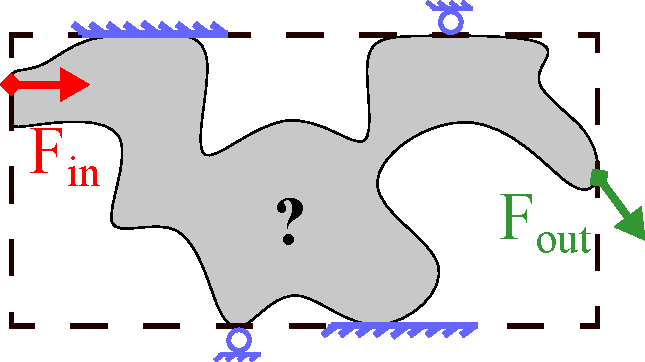
\includegraphics[width=0.5\columnwidth]{images/chap5/TOM-wp.pdf}
    \caption{Basic design problem for compliant mechanisms.}
    \label{fig:ComplProb}
\end{figure}

\subsection{Density-Based Topology Optimization}
The basic concept being topology optimisation consists of investigating the distribution of material inside a discretised design space while trying to improve a certain specified objective function. The design variables applied in this density-based approach optimisation are artificial densities $\ArtDen$ that describe the proportion of the material, $0<\ArtDen_\text{min} \leq \ArtDen \leq 1$, an individual domain space is filled with. The lower and upper bounds of density range are considered as \textit{full} materials representing fully empty or fully filled elements, respectively. While the densities within the range are defined as \textit{intermediate} materials. Here, this artificial density variable are made continuous to use a gradient-based solver which has the advantage of lower computational time compared to non-gradient based approaches, as shown in the work by \cite{sigmund_usefulness_2011}. In order to avoid mesh-dependent solutions and checker-board patters, the optimisation is regulated. This is achieved with a density filter that limits the length scale, $\FiltRadius$, to a minimum inside the structure, as shown in the worky by \cite{bendsoe_topology_2011}.

Each iteration of the optimisation consists of the following steps. First, the filtered design variables are mapped to a material property using the Material Interpolation Scheme (MIS). This converts the artifical densities into a usable Young's Modulus. Next, the well-known Solid Isotropic Material Penalisation (SIMP), as shown in \cref{eq:SIMP} from the work by \cite{bendsoe_topology_2011}, is implemented. This scheme penalises intermediate materials so as to prevent obtaining a geometry that cannot be manufactured. This is done using a penalty facor $\PenFac$ which continuously increases throughout the optimisation.
\begin{equation} % MIS SIMP
  \YoungModulus_\elem = \MIS(\ArtDen_\elem) = ( \overline{\YoungModulus} - \underline{\YoungModulus} ) \ArtDen_\elem ^\PenFac + \underline{\YoungModulus},
\label{eq:SIMP}
\end{equation}
with $\underline{\YoungModulus}$, $\overline{\YoungModulus}$ the lower and upper bound of $\vec{\YoungModulus} =  [\ \!\! \YoungModulus, \cdots, \YoungModulus_\NDesElem]\ \!\!^\text{T}$ respectively corresponding to the Young's modulus of an "empty" element and a completely filled one. $\NDesElem$ is the number of elements inside the domain.
When the material properties of each element are known, the \textit{Stiffness matrix} $\StiffMat$ of the corresponding structure is constructed. Next, Finite Element Analysis (FEA) is performed to estimate the displacement $\Disp$ of each node under imposed external loads $\Load$ so as to solve the linear elasticity equation: $\StiffMat \Disp = \Load$. The chosen objective function with its associated sensitivity (gradient of the objective function with respect to the design variable) is evaluated using these, aforementioned, displacements. For the following iteration, the sensitivites can, then, be used by the solver to update the design variables. In this case, the Optimality Criteria (OC) scheme from the work by \cite{bendsoe_topology_2011} is used as the solver.

One of the main advantages to this approach to designing compliant SMA elements is the fact that various Open-Source academic codes are available for implementing this structural topology optimisation as shown in the work by \cite{zhu_review_2020} and \cite{talischi_polytop_2012}. Due to ignoring the thermal dependencies of the shape memory effect, the resulting FEA used is similar to that of traditional compliant mechanisms and can thus be easily extended to such generative algorithms by simply changing the objective functions and associated sensitivity.

\subsection{Topology Optimization of Compliant Mechanisms}
The basic principle behind designing a compliant mechanism, as illustrated in \cref{fig:ComplProb}, can be formulated as : "Under an external input force and certain boundary conditions, what is the distribution of material defining the compliant mechanism that transforms the input load to a specific output one?"

At the input and output points, artificial springs are added to simulate the intput work and resistance to the output displacement of the workpiece, respectively, as shown in the work by \cite{alonso_topology_2014}. In the final geometry, these springs are removed and are only present during the design process. Regarding the objective function that governs the final design of the compliant mechanism, a formulation that can be extended to Multi-Input Multi-Outputs (MIMO), is implemented based on various strain energies as shown in the work by \cite{alonso_topology_2014}.

An objective function based upon the mutual strain energy between the input and output is chosen. This permits to distribute the strain throughout the structure and avoid to have only \textit{de facto} (single point) hinges responsible for the compliant behaviour. Ideally, the maximum volume of the structure should be deformed to harvest as maximum work, when the alloy is heated and experiences the shape memory effect. Here, the objective function is built using three different types of strain energies. First, there is the input strain energy $\EStrain_\text{in}$, that is present when only an input load $\Load_\text{in}$ is applied and result in some nodal displacements $\Disp_\text{in}$. Similarly, the output strain energy $\EStrain_\text{out}$, is present when only a dummy unit load $\Load_\text{out}$ is applied at the output port resulting in nodal displacements $\Disp_\text{out}$. Finally, the Mutual Potential Energy (MPE) or mutual strain energy $\EStrain_\text{mut}$ can be built with the two previous nodal displacements. The objective function is chosen as a ratio of these three energies due to its non-dimensional aspect and due to the fact that the desired input and output displacements are indirectly accounted for. Here, since the problem is formulated as a minimisation, a minus signed is placed before the chosen ratio to maximise the MPE as follows :
\begin{equation}
    \ObjFct = - \frac{\EStrain_\text{mut}}{\EStrain_\text{in} + \EStrain_\text{out}} = -\frac{{\Disp _\text{out}}^\text{T} \StiffMat \Disp_\text{int}}{\frac{1}{2} {\Disp_\text{out}}^\text{T} \StiffMat \Disp_\text{out} + \frac{1}{2} {\Disp_\text{in}}^\text{T} \StiffMat \Disp_\text{in}}.
\end{equation}
Lastly, two separate FEAs are performed to evaluate the chosen objective: $\StiffMat \Disp_\text{in} = \Load_\text{in}$ and  $\StiffMat \Disp_\text{out} = \Load_\text{out}$.

The current objective governing the design of the generated compliant mechanisms made of \textit{conventional} linear material, can be extended to generating design for mechanisms made from SMAs. This is due to the fact that, as previously mentioned, the algorithm tends to distribute the strain throughout the structure which will indirectly allow a large portion of the material to be activated if made from SMA. The optimisation problem, as formulated in \cref{eq:OptProblem}, consists of the minimisation of the objective function $\ObjFct$ subject to the limitation of the infill $\Volume^{\ast}$ of the design domain's volume, with $\VolumeElem_\elem$ the volume of element $\elem$.

\begin{alignat}{2} % Optimization problem
  \label{eq:OptProblem}
  &\underset{\vec{\ArtDen}}{\text{min}} : \quad        &&\ObjFct(\vec{\Disp_\text{in}},\vec{\Disp_\text{out}},\vec{\YoungModulus}) \notag \\
  &\text{s.t. :}            &&  \StiffMat \Disp_\text{in} = \Load_\text{in}         \notag       \\
  &                         &&  \StiffMat \Disp_\text{out} = \Load_\text{out}                \\
  &                         && \Volume < \Volume^{\ast} \text{,   with } \Volume = (\sum_{\elem=1}^{\NDesElem} \ArtDen_\elem \cdot \VolumeElem_\elem) / (\sum_{\elem=1}^{\NDesElem} \VolumeElem_\elem)   \notag      \\
  &                         && \vec{\YoungModulus} = \MIS(\vec{\ArtDen})    \quad \;     0<\ArtDen_\text{min}    \leqslant \ArtDen    \leqslant 1.     \notag
\end{alignat}

In \cref{fig:Invert_ProbFinal}, the basic design problem is displayed using the common force inverter scenario. Due to the symmetry of the problem, the domain space can be restricted to half the surface while adding rolling supports at the symmetry axis. In \cref{fig:ForceInverter_evol}, the evolution of the optimisation can be observed. Here the domain space is uniformly initialised with intermediate materials such that the volume limitation is satisfied so as to have the design converge to a solution that is only composed of full materials.

\section{Benchmark problems}
Before designing complex multi-output compliant SMA elements, the shape memory effect of the generated geometries must be validated. In this regard, a common practice is to use some traditional benchmark problems. The problems, while being simple problems, can be used to validate the generated designs using a commercially available Finite Element Modelling (FEM) software such as ANSYS\textsuperscript{\textregistered}. Using an FEM, the shape memory effect of the generated topologies can be simulated, verifying the efficiency of the algorithm for designing compliant SMA mechanisms.

The proposed design method is applied to three benchmark problems : an inverter, a crimper, and a gripper. They are all fixed at their bottom and top left corners (which corresponds to ideal pivots) but each have their own input and output forces. The design problems and the resulting geometries are shown in \todocite. This half domain space has been discretised into $10^4$ elements and the design variables are initialised uniformly with a volume fraction constraint of 30\%. The stiffness of each artificial spring is equal to 0.1 and the input forces are equal to 1. When run on a Windows workstation with an Intel i7 3.6 GHz, 8-core processor and 32 GB of memory, the complete process takes less than 1 minute to converge to solution. It is important to note that the computational time would have been significantly higher if a non-linear and multi-physic analysis was executed. Due to the short computational time, this design method can be extended to 3-Dimensional problems.

\begin{figure}[h!]
    \centering
    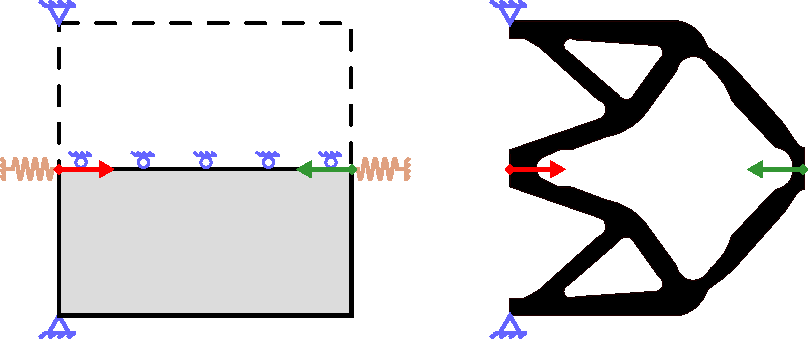
\includegraphics[width=0.7\columnwidth]{images/chap5/Inverter_Schematic_FinalCAD.pdf}
    \caption{Inverter: Design problem (left), Interpolated final topology (right). Input force is shown in red while the output force is shown green.}
    \label{fig:Invert_ProbFinal}
\end{figure}

\begin{figure}[h!]
    \centering
     \begin{subfigure}[t]{0.24\columnwidth} % The width should be scaled to the desired one depending on the number and sizes of sub-figures
     \centering
		   
\includegraphics[width=\textwidth]{images/chap5/Inverter_evo_00.png} % the textwidth will correspond to the one provide by the subfigure width
    %  \caption{Initial}
 \end{subfigure}
%  \hspace{0.2cm}
%  \begin{subfigure}[t]{0.24\columnwidth} % the [t] extension aligns the figure with their tops
%      \centering
% 		   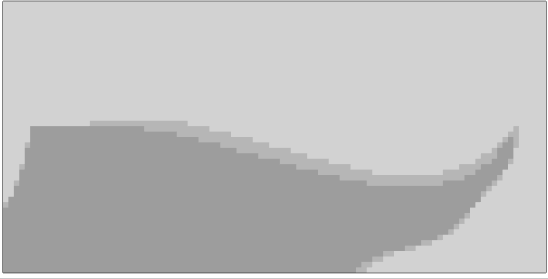
\includegraphics[width=\textwidth]{Inverter_evo_01.png} % the textwidth will correspond to the one provide by the subfigure width
%     %  \caption{Iteration 2}
%  \end{subfigure}
 \hspace{0.2cm}
 \begin{subfigure}[t]{0.24\columnwidth} % the [t] extension aligns the figure with their tops
     \centering
		   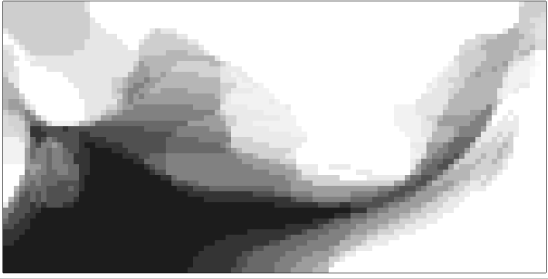
\includegraphics[width=\textwidth]{images/chap5/Inverter_evo_02.png} % the textwidth will correspond to the one provide by the subfigure width
    %  \caption{Iteration 8}
 \end{subfigure}
 \hspace{0.2cm}
 \begin{subfigure}[t]{0.24\columnwidth} % the [t] extension aligns the figure with their tops
     \centering
		   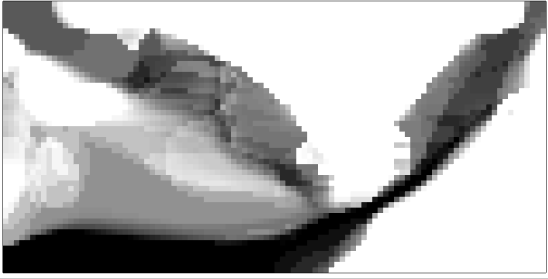
\includegraphics[width=\textwidth]{images/chap5/Inverter_evo_03.png} % the textwidth will correspond to the one provide by the subfigure width
    %  \caption{Iteration 21}
 \end{subfigure}
 \medbreak
 \begin{subfigure}[t]{0.24\columnwidth} % the [t] extension aligns the figure with their tops
     \centering
		   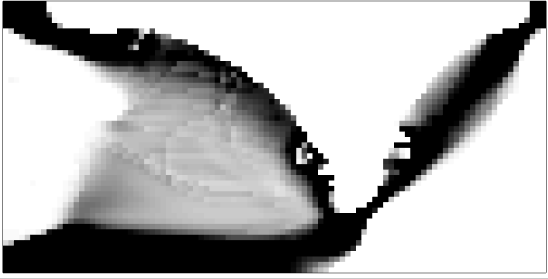
\includegraphics[width=\textwidth]{images/chap5/Inverter_evo_04.png} % the textwidth will correspond to the one provide by the subfigure width
    %  \caption{Iteration 57}
 \end{subfigure}
 \hspace{0.2cm}
 \begin{subfigure}[t]{0.25\columnwidth} % the [t] extension aligns the figure with their tops
     \centering
		   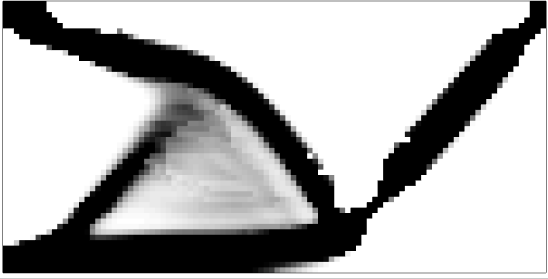
\includegraphics[width=\textwidth]{images/chap5/Inverter_evo_05.png} % the textwidth will correspond to the one provide by the subfigure width
    %  \caption{Iteration 98}
 \end{subfigure}
  \hspace{0.2cm}
 \begin{subfigure}[t]{0.25\columnwidth} % the [t] extension aligns the figure with their tops
     \centering
		   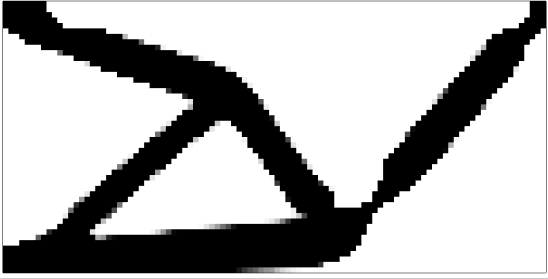
\includegraphics[width=\textwidth]{images/chap5/Inverter_evo_final.png} % the textwidth will correspond to the one provide by the subfigure width
    %  \caption{Iteration 133}
 \end{subfigure}

    \caption{Evolution of the inverter design throughout the optimization. The grayscale represent the value of the filtered artificial density.}
    \label{fig:ForceInverter_evol}
\end{figure}

\begin{figure}[h!]
    \centering
    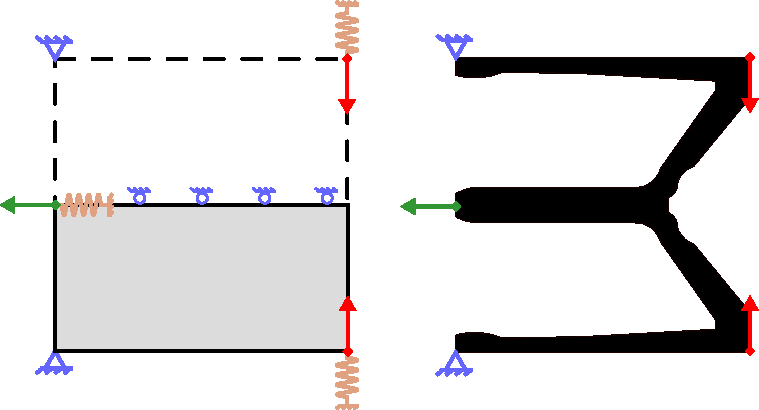
\includegraphics[width=0.7\columnwidth]{images/chap5/Crimper_Schematic_FinalCAD.pdf}
    \caption{Crimper: Design problem (left), Interpolated final topology (right). Input force is shown in red while the output force is shown green.}
    \label{fig:Crimper_ProbFinal}
\end{figure}
\begin{figure}[h!]
    \centering
    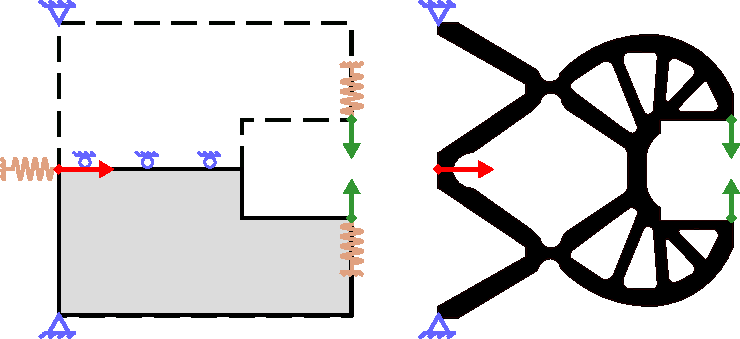
\includegraphics[width=0.7\columnwidth]{images/chap5/Gripper_Schematic_FinalCAD.pdf}
    \caption{Gripper: Design problem (left), Interpolated final topology (right). Input force is shown in red while the output force is shown green.}
    \label{fig:Gripper_ProbFinal}
\end{figure}

Here, in the hopes of validating the shape memory effect, a four time-step simulation is constructed. The four different simulated steps can be seen in \todocite. Here, the figures represent the results of the FEM simulation for each benchmark problem. The simulation consists of first applying an input displacement which generates a displacement at the output, $\varepsilon_\text{loaded}$. If the entire structure is sufficiently strained to undergo the detwinning process, as explained in chapter \todocite, the structure will keep its deformed shape when the input displacement constraint is released. However, as some areas of the compliant structure does not undergo detwinning, a portion of the strain will be lost when the constraint is released. Thus, the observed strain at the output will decrease to $\varepsilon_\text{free}$. During the third time step, the structure is heated to activate the shape memory effect and force the structure to revert back to its original shape where all the strain is recovered. Finally, the structure is allowed to cool down and return the material back to its martensitic phase.

\begin{figure}[hbt!]
    \centering
    % !TEX root = ../sethomas_thesis_main.tex
\documentclass[border=1mm,
               class=article
               preview]{standalone}
\usepackage{tikz}
\begin{document}
\begin{tikzpicture}
    \node[anchor=south west,inner sep=0] (graph) at (0,0) {\resizebox{\columnwidth}{!}{%% Creator: Matplotlib, PGF backend
%%
%% To include the figure in your LaTeX document, write
%%   \input{<filename>.pgf}
%%
%% Make sure the required packages are loaded in your preamble
%%   \usepackage{pgf}
%%
%% and, on pdftex
%%   \usepackage[utf8]{inputenc}\DeclareUnicodeCharacter{2212}{-}
%%
%% or, on luatex and xetex
%%   \usepackage{unicode-math}
%%
%% Figures using additional raster images can only be included by \input if
%% they are in the same directory as the main LaTeX file. For loading figures
%% from other directories you can use the `import` package
%%   \usepackage{import}
%%
%% and then include the figures with
%%   \import{<path to file>}{<filename>.pgf}
%%
%% Matplotlib used the following preamble
%%
\begingroup%
\makeatletter%
\begin{pgfpicture}%
\pgfpathrectangle{\pgfpointorigin}{\pgfqpoint{8.602007in}{4.649344in}}%
\pgfusepath{use as bounding box, clip}%
\begin{pgfscope}%
\pgfsetbuttcap%
\pgfsetmiterjoin%
\pgfsetlinewidth{0.000000pt}%
\definecolor{currentstroke}{rgb}{0.000000,0.000000,0.000000}%
\pgfsetstrokecolor{currentstroke}%
\pgfsetstrokeopacity{0.000000}%
\pgfsetdash{}{0pt}%
\pgfpathmoveto{\pgfqpoint{0.000000in}{0.000000in}}%
\pgfpathlineto{\pgfqpoint{8.602007in}{0.000000in}}%
\pgfpathlineto{\pgfqpoint{8.602007in}{4.649344in}}%
\pgfpathlineto{\pgfqpoint{0.000000in}{4.649344in}}%
\pgfpathclose%
\pgfusepath{}%
\end{pgfscope}%
\begin{pgfscope}%
\pgfsetbuttcap%
\pgfsetmiterjoin%
\pgfsetlinewidth{0.000000pt}%
\definecolor{currentstroke}{rgb}{0.000000,0.000000,0.000000}%
\pgfsetstrokecolor{currentstroke}%
\pgfsetstrokeopacity{0.000000}%
\pgfsetdash{}{0pt}%
\pgfpathmoveto{\pgfqpoint{0.717284in}{3.271659in}}%
\pgfpathlineto{\pgfqpoint{8.467284in}{3.271659in}}%
\pgfpathlineto{\pgfqpoint{8.467284in}{4.404012in}}%
\pgfpathlineto{\pgfqpoint{0.717284in}{4.404012in}}%
\pgfpathclose%
\pgfusepath{}%
\end{pgfscope}%
\begin{pgfscope}%
\pgfpathrectangle{\pgfqpoint{0.717284in}{3.271659in}}{\pgfqpoint{7.750000in}{1.132353in}}%
\pgfusepath{clip}%
\pgfsetbuttcap%
\pgfsetroundjoin%
\pgfsetlinewidth{0.803000pt}%
\definecolor{currentstroke}{rgb}{0.690196,0.690196,0.690196}%
\pgfsetstrokecolor{currentstroke}%
\pgfsetdash{{2.960000pt}{1.280000pt}}{0.000000pt}%
\pgfpathmoveto{\pgfqpoint{2.654784in}{3.271659in}}%
\pgfpathlineto{\pgfqpoint{2.654784in}{4.404012in}}%
\pgfusepath{stroke}%
\end{pgfscope}%
\begin{pgfscope}%
\pgfsetbuttcap%
\pgfsetroundjoin%
\definecolor{currentfill}{rgb}{0.000000,0.000000,0.000000}%
\pgfsetfillcolor{currentfill}%
\pgfsetlinewidth{0.803000pt}%
\definecolor{currentstroke}{rgb}{0.000000,0.000000,0.000000}%
\pgfsetstrokecolor{currentstroke}%
\pgfsetdash{}{0pt}%
\pgfsys@defobject{currentmarker}{\pgfqpoint{0.000000in}{-0.048611in}}{\pgfqpoint{0.000000in}{0.000000in}}{%
\pgfpathmoveto{\pgfqpoint{0.000000in}{0.000000in}}%
\pgfpathlineto{\pgfqpoint{0.000000in}{-0.048611in}}%
\pgfusepath{stroke,fill}%
}%
\begin{pgfscope}%
\pgfsys@transformshift{2.654784in}{3.271659in}%
\pgfsys@useobject{currentmarker}{}%
\end{pgfscope}%
\end{pgfscope}%
\begin{pgfscope}%
\pgfpathrectangle{\pgfqpoint{0.717284in}{3.271659in}}{\pgfqpoint{7.750000in}{1.132353in}}%
\pgfusepath{clip}%
\pgfsetbuttcap%
\pgfsetroundjoin%
\pgfsetlinewidth{0.803000pt}%
\definecolor{currentstroke}{rgb}{0.690196,0.690196,0.690196}%
\pgfsetstrokecolor{currentstroke}%
\pgfsetdash{{2.960000pt}{1.280000pt}}{0.000000pt}%
\pgfpathmoveto{\pgfqpoint{4.592284in}{3.271659in}}%
\pgfpathlineto{\pgfqpoint{4.592284in}{4.404012in}}%
\pgfusepath{stroke}%
\end{pgfscope}%
\begin{pgfscope}%
\pgfsetbuttcap%
\pgfsetroundjoin%
\definecolor{currentfill}{rgb}{0.000000,0.000000,0.000000}%
\pgfsetfillcolor{currentfill}%
\pgfsetlinewidth{0.803000pt}%
\definecolor{currentstroke}{rgb}{0.000000,0.000000,0.000000}%
\pgfsetstrokecolor{currentstroke}%
\pgfsetdash{}{0pt}%
\pgfsys@defobject{currentmarker}{\pgfqpoint{0.000000in}{-0.048611in}}{\pgfqpoint{0.000000in}{0.000000in}}{%
\pgfpathmoveto{\pgfqpoint{0.000000in}{0.000000in}}%
\pgfpathlineto{\pgfqpoint{0.000000in}{-0.048611in}}%
\pgfusepath{stroke,fill}%
}%
\begin{pgfscope}%
\pgfsys@transformshift{4.592284in}{3.271659in}%
\pgfsys@useobject{currentmarker}{}%
\end{pgfscope}%
\end{pgfscope}%
\begin{pgfscope}%
\pgfpathrectangle{\pgfqpoint{0.717284in}{3.271659in}}{\pgfqpoint{7.750000in}{1.132353in}}%
\pgfusepath{clip}%
\pgfsetbuttcap%
\pgfsetroundjoin%
\pgfsetlinewidth{0.803000pt}%
\definecolor{currentstroke}{rgb}{0.690196,0.690196,0.690196}%
\pgfsetstrokecolor{currentstroke}%
\pgfsetdash{{2.960000pt}{1.280000pt}}{0.000000pt}%
\pgfpathmoveto{\pgfqpoint{6.529784in}{3.271659in}}%
\pgfpathlineto{\pgfqpoint{6.529784in}{4.404012in}}%
\pgfusepath{stroke}%
\end{pgfscope}%
\begin{pgfscope}%
\pgfsetbuttcap%
\pgfsetroundjoin%
\definecolor{currentfill}{rgb}{0.000000,0.000000,0.000000}%
\pgfsetfillcolor{currentfill}%
\pgfsetlinewidth{0.803000pt}%
\definecolor{currentstroke}{rgb}{0.000000,0.000000,0.000000}%
\pgfsetstrokecolor{currentstroke}%
\pgfsetdash{}{0pt}%
\pgfsys@defobject{currentmarker}{\pgfqpoint{0.000000in}{-0.048611in}}{\pgfqpoint{0.000000in}{0.000000in}}{%
\pgfpathmoveto{\pgfqpoint{0.000000in}{0.000000in}}%
\pgfpathlineto{\pgfqpoint{0.000000in}{-0.048611in}}%
\pgfusepath{stroke,fill}%
}%
\begin{pgfscope}%
\pgfsys@transformshift{6.529784in}{3.271659in}%
\pgfsys@useobject{currentmarker}{}%
\end{pgfscope}%
\end{pgfscope}%
\begin{pgfscope}%
\pgfpathrectangle{\pgfqpoint{0.717284in}{3.271659in}}{\pgfqpoint{7.750000in}{1.132353in}}%
\pgfusepath{clip}%
\pgfsetbuttcap%
\pgfsetroundjoin%
\pgfsetlinewidth{0.803000pt}%
\definecolor{currentstroke}{rgb}{0.690196,0.690196,0.690196}%
\pgfsetstrokecolor{currentstroke}%
\pgfsetdash{{2.960000pt}{1.280000pt}}{0.000000pt}%
\pgfpathmoveto{\pgfqpoint{8.467284in}{3.271659in}}%
\pgfpathlineto{\pgfqpoint{8.467284in}{4.404012in}}%
\pgfusepath{stroke}%
\end{pgfscope}%
\begin{pgfscope}%
\pgfsetbuttcap%
\pgfsetroundjoin%
\definecolor{currentfill}{rgb}{0.000000,0.000000,0.000000}%
\pgfsetfillcolor{currentfill}%
\pgfsetlinewidth{0.803000pt}%
\definecolor{currentstroke}{rgb}{0.000000,0.000000,0.000000}%
\pgfsetstrokecolor{currentstroke}%
\pgfsetdash{}{0pt}%
\pgfsys@defobject{currentmarker}{\pgfqpoint{0.000000in}{-0.048611in}}{\pgfqpoint{0.000000in}{0.000000in}}{%
\pgfpathmoveto{\pgfqpoint{0.000000in}{0.000000in}}%
\pgfpathlineto{\pgfqpoint{0.000000in}{-0.048611in}}%
\pgfusepath{stroke,fill}%
}%
\begin{pgfscope}%
\pgfsys@transformshift{8.467284in}{3.271659in}%
\pgfsys@useobject{currentmarker}{}%
\end{pgfscope}%
\end{pgfscope}%
\begin{pgfscope}%
\pgfpathrectangle{\pgfqpoint{0.717284in}{3.271659in}}{\pgfqpoint{7.750000in}{1.132353in}}%
\pgfusepath{clip}%
\pgfsetbuttcap%
\pgfsetroundjoin%
\pgfsetlinewidth{0.803000pt}%
\definecolor{currentstroke}{rgb}{0.690196,0.690196,0.690196}%
\pgfsetstrokecolor{currentstroke}%
\pgfsetdash{{2.960000pt}{1.280000pt}}{0.000000pt}%
\pgfpathmoveto{\pgfqpoint{0.717284in}{3.323129in}}%
\pgfpathlineto{\pgfqpoint{8.467284in}{3.323129in}}%
\pgfusepath{stroke}%
\end{pgfscope}%
\begin{pgfscope}%
\pgfsetbuttcap%
\pgfsetroundjoin%
\definecolor{currentfill}{rgb}{0.000000,0.000000,0.000000}%
\pgfsetfillcolor{currentfill}%
\pgfsetlinewidth{0.803000pt}%
\definecolor{currentstroke}{rgb}{0.000000,0.000000,0.000000}%
\pgfsetstrokecolor{currentstroke}%
\pgfsetdash{}{0pt}%
\pgfsys@defobject{currentmarker}{\pgfqpoint{-0.048611in}{0.000000in}}{\pgfqpoint{-0.000000in}{0.000000in}}{%
\pgfpathmoveto{\pgfqpoint{-0.000000in}{0.000000in}}%
\pgfpathlineto{\pgfqpoint{-0.048611in}{0.000000in}}%
\pgfusepath{stroke,fill}%
}%
\begin{pgfscope}%
\pgfsys@transformshift{0.717284in}{3.323129in}%
\pgfsys@useobject{currentmarker}{}%
\end{pgfscope}%
\end{pgfscope}%
\begin{pgfscope}%
\definecolor{textcolor}{rgb}{0.000000,0.000000,0.000000}%
\pgfsetstrokecolor{textcolor}%
\pgfsetfillcolor{textcolor}%
\pgftext[x=0.481173in, y=3.274904in, left, base]{\color{textcolor}\rmfamily\fontsize{10.000000}{12.000000}\selectfont \(\displaystyle {22}\)}%
\end{pgfscope}%
\begin{pgfscope}%
\pgfpathrectangle{\pgfqpoint{0.717284in}{3.271659in}}{\pgfqpoint{7.750000in}{1.132353in}}%
\pgfusepath{clip}%
\pgfsetbuttcap%
\pgfsetroundjoin%
\pgfsetlinewidth{0.803000pt}%
\definecolor{currentstroke}{rgb}{0.690196,0.690196,0.690196}%
\pgfsetstrokecolor{currentstroke}%
\pgfsetdash{{2.960000pt}{1.280000pt}}{0.000000pt}%
\pgfpathmoveto{\pgfqpoint{0.717284in}{4.352541in}}%
\pgfpathlineto{\pgfqpoint{8.467284in}{4.352541in}}%
\pgfusepath{stroke}%
\end{pgfscope}%
\begin{pgfscope}%
\pgfsetbuttcap%
\pgfsetroundjoin%
\definecolor{currentfill}{rgb}{0.000000,0.000000,0.000000}%
\pgfsetfillcolor{currentfill}%
\pgfsetlinewidth{0.803000pt}%
\definecolor{currentstroke}{rgb}{0.000000,0.000000,0.000000}%
\pgfsetstrokecolor{currentstroke}%
\pgfsetdash{}{0pt}%
\pgfsys@defobject{currentmarker}{\pgfqpoint{-0.048611in}{0.000000in}}{\pgfqpoint{-0.000000in}{0.000000in}}{%
\pgfpathmoveto{\pgfqpoint{-0.000000in}{0.000000in}}%
\pgfpathlineto{\pgfqpoint{-0.048611in}{0.000000in}}%
\pgfusepath{stroke,fill}%
}%
\begin{pgfscope}%
\pgfsys@transformshift{0.717284in}{4.352541in}%
\pgfsys@useobject{currentmarker}{}%
\end{pgfscope}%
\end{pgfscope}%
\begin{pgfscope}%
\definecolor{textcolor}{rgb}{0.000000,0.000000,0.000000}%
\pgfsetstrokecolor{textcolor}%
\pgfsetfillcolor{textcolor}%
\pgftext[x=0.411728in, y=4.304316in, left, base]{\color{textcolor}\rmfamily\fontsize{10.000000}{12.000000}\selectfont \(\displaystyle {160}\)}%
\end{pgfscope}%
\begin{pgfscope}%
\definecolor{textcolor}{rgb}{0.000000,0.000000,0.000000}%
\pgfsetstrokecolor{textcolor}%
\pgfsetfillcolor{textcolor}%
\pgftext[x=0.356173in,y=3.837835in,,bottom,rotate=90.000000]{\color{textcolor}\rmfamily\fontsize{12.000000}{14.400000}\bfseries\selectfont Temperature [°C]}%
\end{pgfscope}%
\begin{pgfscope}%
\pgfpathrectangle{\pgfqpoint{0.717284in}{3.271659in}}{\pgfqpoint{7.750000in}{1.132353in}}%
\pgfusepath{clip}%
\pgfsetbuttcap%
\pgfsetroundjoin%
\pgfsetlinewidth{3.011250pt}%
\definecolor{currentstroke}{rgb}{0.450980,0.670588,1.000000}%
\pgfsetstrokecolor{currentstroke}%
\pgfsetdash{{3.000000pt}{4.950000pt}}{0.000000pt}%
\pgfpathmoveto{\pgfqpoint{0.717284in}{3.323129in}}%
\pgfpathlineto{\pgfqpoint{4.592284in}{3.323129in}}%
\pgfpathlineto{\pgfqpoint{5.754978in}{3.940851in}}%
\pgfpathlineto{\pgfqpoint{5.756722in}{3.941000in}}%
\pgfpathlineto{\pgfqpoint{6.529784in}{4.352541in}}%
\pgfpathlineto{\pgfqpoint{6.529784in}{4.352541in}}%
\pgfpathlineto{\pgfqpoint{8.467284in}{3.323129in}}%
\pgfpathlineto{\pgfqpoint{8.467284in}{3.323129in}}%
\pgfusepath{stroke}%
\end{pgfscope}%
\begin{pgfscope}%
\pgfsetrectcap%
\pgfsetmiterjoin%
\pgfsetlinewidth{0.803000pt}%
\definecolor{currentstroke}{rgb}{0.000000,0.000000,0.000000}%
\pgfsetstrokecolor{currentstroke}%
\pgfsetdash{}{0pt}%
\pgfpathmoveto{\pgfqpoint{0.717284in}{3.271659in}}%
\pgfpathlineto{\pgfqpoint{0.717284in}{4.404012in}}%
\pgfusepath{stroke}%
\end{pgfscope}%
\begin{pgfscope}%
\pgfsetrectcap%
\pgfsetmiterjoin%
\pgfsetlinewidth{0.803000pt}%
\definecolor{currentstroke}{rgb}{0.000000,0.000000,0.000000}%
\pgfsetstrokecolor{currentstroke}%
\pgfsetdash{}{0pt}%
\pgfpathmoveto{\pgfqpoint{8.467284in}{3.271659in}}%
\pgfpathlineto{\pgfqpoint{8.467284in}{4.404012in}}%
\pgfusepath{stroke}%
\end{pgfscope}%
\begin{pgfscope}%
\pgfsetrectcap%
\pgfsetmiterjoin%
\pgfsetlinewidth{0.803000pt}%
\definecolor{currentstroke}{rgb}{0.000000,0.000000,0.000000}%
\pgfsetstrokecolor{currentstroke}%
\pgfsetdash{}{0pt}%
\pgfpathmoveto{\pgfqpoint{0.717284in}{3.271659in}}%
\pgfpathlineto{\pgfqpoint{8.467284in}{3.271659in}}%
\pgfusepath{stroke}%
\end{pgfscope}%
\begin{pgfscope}%
\pgfsetrectcap%
\pgfsetmiterjoin%
\pgfsetlinewidth{0.803000pt}%
\definecolor{currentstroke}{rgb}{0.000000,0.000000,0.000000}%
\pgfsetstrokecolor{currentstroke}%
\pgfsetdash{}{0pt}%
\pgfpathmoveto{\pgfqpoint{0.717284in}{4.404012in}}%
\pgfpathlineto{\pgfqpoint{8.467284in}{4.404012in}}%
\pgfusepath{stroke}%
\end{pgfscope}%
\begin{pgfscope}%
\pgfsetbuttcap%
\pgfsetmiterjoin%
\pgfsetlinewidth{0.000000pt}%
\definecolor{currentstroke}{rgb}{0.000000,0.000000,0.000000}%
\pgfsetstrokecolor{currentstroke}%
\pgfsetstrokeopacity{0.000000}%
\pgfsetdash{}{0pt}%
\pgfpathmoveto{\pgfqpoint{0.717284in}{1.912835in}}%
\pgfpathlineto{\pgfqpoint{8.467284in}{1.912835in}}%
\pgfpathlineto{\pgfqpoint{8.467284in}{3.045188in}}%
\pgfpathlineto{\pgfqpoint{0.717284in}{3.045188in}}%
\pgfpathclose%
\pgfusepath{}%
\end{pgfscope}%
\begin{pgfscope}%
\pgfpathrectangle{\pgfqpoint{0.717284in}{1.912835in}}{\pgfqpoint{7.750000in}{1.132353in}}%
\pgfusepath{clip}%
\pgfsetbuttcap%
\pgfsetroundjoin%
\pgfsetlinewidth{0.803000pt}%
\definecolor{currentstroke}{rgb}{0.690196,0.690196,0.690196}%
\pgfsetstrokecolor{currentstroke}%
\pgfsetdash{{2.960000pt}{1.280000pt}}{0.000000pt}%
\pgfpathmoveto{\pgfqpoint{2.654784in}{1.912835in}}%
\pgfpathlineto{\pgfqpoint{2.654784in}{3.045188in}}%
\pgfusepath{stroke}%
\end{pgfscope}%
\begin{pgfscope}%
\pgfsetbuttcap%
\pgfsetroundjoin%
\definecolor{currentfill}{rgb}{0.000000,0.000000,0.000000}%
\pgfsetfillcolor{currentfill}%
\pgfsetlinewidth{0.803000pt}%
\definecolor{currentstroke}{rgb}{0.000000,0.000000,0.000000}%
\pgfsetstrokecolor{currentstroke}%
\pgfsetdash{}{0pt}%
\pgfsys@defobject{currentmarker}{\pgfqpoint{0.000000in}{-0.048611in}}{\pgfqpoint{0.000000in}{0.000000in}}{%
\pgfpathmoveto{\pgfqpoint{0.000000in}{0.000000in}}%
\pgfpathlineto{\pgfqpoint{0.000000in}{-0.048611in}}%
\pgfusepath{stroke,fill}%
}%
\begin{pgfscope}%
\pgfsys@transformshift{2.654784in}{1.912835in}%
\pgfsys@useobject{currentmarker}{}%
\end{pgfscope}%
\end{pgfscope}%
\begin{pgfscope}%
\pgfpathrectangle{\pgfqpoint{0.717284in}{1.912835in}}{\pgfqpoint{7.750000in}{1.132353in}}%
\pgfusepath{clip}%
\pgfsetbuttcap%
\pgfsetroundjoin%
\pgfsetlinewidth{0.803000pt}%
\definecolor{currentstroke}{rgb}{0.690196,0.690196,0.690196}%
\pgfsetstrokecolor{currentstroke}%
\pgfsetdash{{2.960000pt}{1.280000pt}}{0.000000pt}%
\pgfpathmoveto{\pgfqpoint{4.592284in}{1.912835in}}%
\pgfpathlineto{\pgfqpoint{4.592284in}{3.045188in}}%
\pgfusepath{stroke}%
\end{pgfscope}%
\begin{pgfscope}%
\pgfsetbuttcap%
\pgfsetroundjoin%
\definecolor{currentfill}{rgb}{0.000000,0.000000,0.000000}%
\pgfsetfillcolor{currentfill}%
\pgfsetlinewidth{0.803000pt}%
\definecolor{currentstroke}{rgb}{0.000000,0.000000,0.000000}%
\pgfsetstrokecolor{currentstroke}%
\pgfsetdash{}{0pt}%
\pgfsys@defobject{currentmarker}{\pgfqpoint{0.000000in}{-0.048611in}}{\pgfqpoint{0.000000in}{0.000000in}}{%
\pgfpathmoveto{\pgfqpoint{0.000000in}{0.000000in}}%
\pgfpathlineto{\pgfqpoint{0.000000in}{-0.048611in}}%
\pgfusepath{stroke,fill}%
}%
\begin{pgfscope}%
\pgfsys@transformshift{4.592284in}{1.912835in}%
\pgfsys@useobject{currentmarker}{}%
\end{pgfscope}%
\end{pgfscope}%
\begin{pgfscope}%
\pgfpathrectangle{\pgfqpoint{0.717284in}{1.912835in}}{\pgfqpoint{7.750000in}{1.132353in}}%
\pgfusepath{clip}%
\pgfsetbuttcap%
\pgfsetroundjoin%
\pgfsetlinewidth{0.803000pt}%
\definecolor{currentstroke}{rgb}{0.690196,0.690196,0.690196}%
\pgfsetstrokecolor{currentstroke}%
\pgfsetdash{{2.960000pt}{1.280000pt}}{0.000000pt}%
\pgfpathmoveto{\pgfqpoint{6.529784in}{1.912835in}}%
\pgfpathlineto{\pgfqpoint{6.529784in}{3.045188in}}%
\pgfusepath{stroke}%
\end{pgfscope}%
\begin{pgfscope}%
\pgfsetbuttcap%
\pgfsetroundjoin%
\definecolor{currentfill}{rgb}{0.000000,0.000000,0.000000}%
\pgfsetfillcolor{currentfill}%
\pgfsetlinewidth{0.803000pt}%
\definecolor{currentstroke}{rgb}{0.000000,0.000000,0.000000}%
\pgfsetstrokecolor{currentstroke}%
\pgfsetdash{}{0pt}%
\pgfsys@defobject{currentmarker}{\pgfqpoint{0.000000in}{-0.048611in}}{\pgfqpoint{0.000000in}{0.000000in}}{%
\pgfpathmoveto{\pgfqpoint{0.000000in}{0.000000in}}%
\pgfpathlineto{\pgfqpoint{0.000000in}{-0.048611in}}%
\pgfusepath{stroke,fill}%
}%
\begin{pgfscope}%
\pgfsys@transformshift{6.529784in}{1.912835in}%
\pgfsys@useobject{currentmarker}{}%
\end{pgfscope}%
\end{pgfscope}%
\begin{pgfscope}%
\pgfpathrectangle{\pgfqpoint{0.717284in}{1.912835in}}{\pgfqpoint{7.750000in}{1.132353in}}%
\pgfusepath{clip}%
\pgfsetbuttcap%
\pgfsetroundjoin%
\pgfsetlinewidth{0.803000pt}%
\definecolor{currentstroke}{rgb}{0.690196,0.690196,0.690196}%
\pgfsetstrokecolor{currentstroke}%
\pgfsetdash{{2.960000pt}{1.280000pt}}{0.000000pt}%
\pgfpathmoveto{\pgfqpoint{8.467284in}{1.912835in}}%
\pgfpathlineto{\pgfqpoint{8.467284in}{3.045188in}}%
\pgfusepath{stroke}%
\end{pgfscope}%
\begin{pgfscope}%
\pgfsetbuttcap%
\pgfsetroundjoin%
\definecolor{currentfill}{rgb}{0.000000,0.000000,0.000000}%
\pgfsetfillcolor{currentfill}%
\pgfsetlinewidth{0.803000pt}%
\definecolor{currentstroke}{rgb}{0.000000,0.000000,0.000000}%
\pgfsetstrokecolor{currentstroke}%
\pgfsetdash{}{0pt}%
\pgfsys@defobject{currentmarker}{\pgfqpoint{0.000000in}{-0.048611in}}{\pgfqpoint{0.000000in}{0.000000in}}{%
\pgfpathmoveto{\pgfqpoint{0.000000in}{0.000000in}}%
\pgfpathlineto{\pgfqpoint{0.000000in}{-0.048611in}}%
\pgfusepath{stroke,fill}%
}%
\begin{pgfscope}%
\pgfsys@transformshift{8.467284in}{1.912835in}%
\pgfsys@useobject{currentmarker}{}%
\end{pgfscope}%
\end{pgfscope}%
\begin{pgfscope}%
\pgfpathrectangle{\pgfqpoint{0.717284in}{1.912835in}}{\pgfqpoint{7.750000in}{1.132353in}}%
\pgfusepath{clip}%
\pgfsetbuttcap%
\pgfsetroundjoin%
\pgfsetlinewidth{0.803000pt}%
\definecolor{currentstroke}{rgb}{0.690196,0.690196,0.690196}%
\pgfsetstrokecolor{currentstroke}%
\pgfsetdash{{2.960000pt}{1.280000pt}}{0.000000pt}%
\pgfpathmoveto{\pgfqpoint{0.717284in}{1.964306in}}%
\pgfpathlineto{\pgfqpoint{8.467284in}{1.964306in}}%
\pgfusepath{stroke}%
\end{pgfscope}%
\begin{pgfscope}%
\pgfsetbuttcap%
\pgfsetroundjoin%
\definecolor{currentfill}{rgb}{0.000000,0.000000,0.000000}%
\pgfsetfillcolor{currentfill}%
\pgfsetlinewidth{0.803000pt}%
\definecolor{currentstroke}{rgb}{0.000000,0.000000,0.000000}%
\pgfsetstrokecolor{currentstroke}%
\pgfsetdash{}{0pt}%
\pgfsys@defobject{currentmarker}{\pgfqpoint{-0.048611in}{0.000000in}}{\pgfqpoint{-0.000000in}{0.000000in}}{%
\pgfpathmoveto{\pgfqpoint{-0.000000in}{0.000000in}}%
\pgfpathlineto{\pgfqpoint{-0.048611in}{0.000000in}}%
\pgfusepath{stroke,fill}%
}%
\begin{pgfscope}%
\pgfsys@transformshift{0.717284in}{1.964306in}%
\pgfsys@useobject{currentmarker}{}%
\end{pgfscope}%
\end{pgfscope}%
\begin{pgfscope}%
\definecolor{textcolor}{rgb}{0.000000,0.000000,0.000000}%
\pgfsetstrokecolor{textcolor}%
\pgfsetfillcolor{textcolor}%
\pgftext[x=0.550617in, y=1.916081in, left, base]{\color{textcolor}\rmfamily\fontsize{10.000000}{12.000000}\selectfont 0}%
\end{pgfscope}%
\begin{pgfscope}%
\pgfpathrectangle{\pgfqpoint{0.717284in}{1.912835in}}{\pgfqpoint{7.750000in}{1.132353in}}%
\pgfusepath{clip}%
\pgfsetbuttcap%
\pgfsetroundjoin%
\pgfsetlinewidth{0.803000pt}%
\definecolor{currentstroke}{rgb}{0.690196,0.690196,0.690196}%
\pgfsetstrokecolor{currentstroke}%
\pgfsetdash{{2.960000pt}{1.280000pt}}{0.000000pt}%
\pgfpathmoveto{\pgfqpoint{0.717284in}{2.763202in}}%
\pgfpathlineto{\pgfqpoint{8.467284in}{2.763202in}}%
\pgfusepath{stroke}%
\end{pgfscope}%
\begin{pgfscope}%
\pgfsetbuttcap%
\pgfsetroundjoin%
\definecolor{currentfill}{rgb}{0.000000,0.000000,0.000000}%
\pgfsetfillcolor{currentfill}%
\pgfsetlinewidth{0.803000pt}%
\definecolor{currentstroke}{rgb}{0.000000,0.000000,0.000000}%
\pgfsetstrokecolor{currentstroke}%
\pgfsetdash{}{0pt}%
\pgfsys@defobject{currentmarker}{\pgfqpoint{-0.048611in}{0.000000in}}{\pgfqpoint{-0.000000in}{0.000000in}}{%
\pgfpathmoveto{\pgfqpoint{-0.000000in}{0.000000in}}%
\pgfpathlineto{\pgfqpoint{-0.048611in}{0.000000in}}%
\pgfusepath{stroke,fill}%
}%
\begin{pgfscope}%
\pgfsys@transformshift{0.717284in}{2.763202in}%
\pgfsys@useobject{currentmarker}{}%
\end{pgfscope}%
\end{pgfscope}%
\begin{pgfscope}%
\definecolor{textcolor}{rgb}{0.000000,0.000000,0.000000}%
\pgfsetstrokecolor{textcolor}%
\pgfsetfillcolor{textcolor}%
\pgftext[x=0.303703in, y=2.714976in, left, base]{\color{textcolor}\rmfamily\fontsize{10.000000}{12.000000}\selectfont 0.078}%
\end{pgfscope}%
\begin{pgfscope}%
\pgfpathrectangle{\pgfqpoint{0.717284in}{1.912835in}}{\pgfqpoint{7.750000in}{1.132353in}}%
\pgfusepath{clip}%
\pgfsetbuttcap%
\pgfsetroundjoin%
\pgfsetlinewidth{0.803000pt}%
\definecolor{currentstroke}{rgb}{0.690196,0.690196,0.690196}%
\pgfsetstrokecolor{currentstroke}%
\pgfsetdash{{2.960000pt}{1.280000pt}}{0.000000pt}%
\pgfpathmoveto{\pgfqpoint{0.717284in}{2.991371in}}%
\pgfpathlineto{\pgfqpoint{8.467284in}{2.991371in}}%
\pgfusepath{stroke}%
\end{pgfscope}%
\begin{pgfscope}%
\pgfsetbuttcap%
\pgfsetroundjoin%
\definecolor{currentfill}{rgb}{0.000000,0.000000,0.000000}%
\pgfsetfillcolor{currentfill}%
\pgfsetlinewidth{0.803000pt}%
\definecolor{currentstroke}{rgb}{0.000000,0.000000,0.000000}%
\pgfsetstrokecolor{currentstroke}%
\pgfsetdash{}{0pt}%
\pgfsys@defobject{currentmarker}{\pgfqpoint{-0.048611in}{0.000000in}}{\pgfqpoint{-0.000000in}{0.000000in}}{%
\pgfpathmoveto{\pgfqpoint{-0.000000in}{0.000000in}}%
\pgfpathlineto{\pgfqpoint{-0.048611in}{0.000000in}}%
\pgfusepath{stroke,fill}%
}%
\begin{pgfscope}%
\pgfsys@transformshift{0.717284in}{2.991371in}%
\pgfsys@useobject{currentmarker}{}%
\end{pgfscope}%
\end{pgfscope}%
\begin{pgfscope}%
\definecolor{textcolor}{rgb}{0.000000,0.000000,0.000000}%
\pgfsetstrokecolor{textcolor}%
\pgfsetfillcolor{textcolor}%
\pgftext[x=0.442592in, y=2.943145in, left, base]{\color{textcolor}\rmfamily\fontsize{10.000000}{12.000000}\selectfont 0.1}%
\end{pgfscope}%
\begin{pgfscope}%
\definecolor{textcolor}{rgb}{0.000000,0.000000,0.000000}%
\pgfsetstrokecolor{textcolor}%
\pgfsetfillcolor{textcolor}%
\pgftext[x=0.248148in,y=2.479012in,,bottom,rotate=90.000000]{\color{textcolor}\rmfamily\fontsize{12.000000}{14.400000}\bfseries\selectfont Input Strain}%
\end{pgfscope}%
\begin{pgfscope}%
\pgfpathrectangle{\pgfqpoint{0.717284in}{1.912835in}}{\pgfqpoint{7.750000in}{1.132353in}}%
\pgfusepath{clip}%
\pgfsetrectcap%
\pgfsetroundjoin%
\pgfsetlinewidth{2.007500pt}%
\definecolor{currentstroke}{rgb}{0.952941,0.078431,0.113725}%
\pgfsetstrokecolor{currentstroke}%
\pgfsetdash{}{0pt}%
\pgfpathmoveto{\pgfqpoint{2.667766in}{2.992503in}}%
\pgfpathlineto{\pgfqpoint{2.936109in}{2.968425in}}%
\pgfpathlineto{\pgfqpoint{3.194378in}{2.944316in}}%
\pgfpathlineto{\pgfqpoint{3.452841in}{2.919147in}}%
\pgfpathlineto{\pgfqpoint{3.581878in}{2.906074in}}%
\pgfpathlineto{\pgfqpoint{3.711109in}{2.892310in}}%
\pgfpathlineto{\pgfqpoint{3.840341in}{2.877559in}}%
\pgfpathlineto{\pgfqpoint{3.969378in}{2.862025in}}%
\pgfpathlineto{\pgfqpoint{4.098609in}{2.845668in}}%
\pgfpathlineto{\pgfqpoint{4.227841in}{2.827663in}}%
\pgfpathlineto{\pgfqpoint{4.356878in}{2.807322in}}%
\pgfpathlineto{\pgfqpoint{4.486109in}{2.784459in}}%
\pgfpathlineto{\pgfqpoint{4.592284in}{2.763243in}}%
\pgfpathlineto{\pgfqpoint{4.957116in}{2.763006in}}%
\pgfpathlineto{\pgfqpoint{5.383366in}{2.762749in}}%
\pgfpathlineto{\pgfqpoint{5.422116in}{2.760340in}}%
\pgfpathlineto{\pgfqpoint{5.460866in}{2.753031in}}%
\pgfpathlineto{\pgfqpoint{5.489928in}{2.746391in}}%
\pgfpathlineto{\pgfqpoint{5.518991in}{2.738146in}}%
\pgfpathlineto{\pgfqpoint{5.540884in}{2.730569in}}%
\pgfpathlineto{\pgfqpoint{5.557159in}{2.723796in}}%
\pgfpathlineto{\pgfqpoint{5.573628in}{2.715169in}}%
\pgfpathlineto{\pgfqpoint{5.585834in}{2.707902in}}%
\pgfpathlineto{\pgfqpoint{5.594941in}{2.701499in}}%
\pgfpathlineto{\pgfqpoint{5.601916in}{2.695857in}}%
\pgfpathlineto{\pgfqpoint{5.608891in}{2.689413in}}%
\pgfpathlineto{\pgfqpoint{5.617803in}{2.678965in}}%
\pgfpathlineto{\pgfqpoint{5.624584in}{2.669597in}}%
\pgfpathlineto{\pgfqpoint{5.627491in}{2.665150in}}%
\pgfpathlineto{\pgfqpoint{5.635241in}{2.651418in}}%
\pgfpathlineto{\pgfqpoint{5.642603in}{2.635678in}}%
\pgfpathlineto{\pgfqpoint{5.652291in}{2.607987in}}%
\pgfpathlineto{\pgfqpoint{5.656941in}{2.592237in}}%
\pgfpathlineto{\pgfqpoint{5.663334in}{2.567068in}}%
\pgfpathlineto{\pgfqpoint{5.671472in}{2.530390in}}%
\pgfpathlineto{\pgfqpoint{5.684647in}{2.462407in}}%
\pgfpathlineto{\pgfqpoint{5.691428in}{2.425575in}}%
\pgfpathlineto{\pgfqpoint{5.708284in}{2.323879in}}%
\pgfpathlineto{\pgfqpoint{5.722234in}{2.231706in}}%
\pgfpathlineto{\pgfqpoint{5.730372in}{2.173647in}}%
\pgfpathlineto{\pgfqpoint{5.737153in}{2.125687in}}%
\pgfpathlineto{\pgfqpoint{5.745291in}{2.064101in}}%
\pgfpathlineto{\pgfqpoint{5.750328in}{2.026356in}}%
\pgfpathlineto{\pgfqpoint{5.754978in}{1.990080in}}%
\pgfpathlineto{\pgfqpoint{5.756722in}{1.964306in}}%
\pgfpathlineto{\pgfqpoint{8.467284in}{1.964306in}}%
\pgfpathlineto{\pgfqpoint{8.467284in}{1.964306in}}%
\pgfusepath{stroke}%
\end{pgfscope}%
\begin{pgfscope}%
\pgfpathrectangle{\pgfqpoint{0.717284in}{1.912835in}}{\pgfqpoint{7.750000in}{1.132353in}}%
\pgfusepath{clip}%
\pgfsetbuttcap%
\pgfsetroundjoin%
\pgfsetlinewidth{3.011250pt}%
\definecolor{currentstroke}{rgb}{0.952941,0.078431,0.113725}%
\pgfsetstrokecolor{currentstroke}%
\pgfsetdash{{3.000000pt}{4.950000pt}}{0.000000pt}%
\pgfpathmoveto{\pgfqpoint{0.730201in}{1.971169in}}%
\pgfpathlineto{\pgfqpoint{0.743117in}{1.978031in}}%
\pgfpathlineto{\pgfqpoint{0.762492in}{1.988325in}}%
\pgfpathlineto{\pgfqpoint{0.781867in}{1.998619in}}%
\pgfpathlineto{\pgfqpoint{0.801242in}{2.008913in}}%
\pgfpathlineto{\pgfqpoint{0.815773in}{2.016634in}}%
\pgfpathlineto{\pgfqpoint{0.830304in}{2.024355in}}%
\pgfpathlineto{\pgfqpoint{0.844836in}{2.032075in}}%
\pgfpathlineto{\pgfqpoint{0.866633in}{2.043656in}}%
\pgfpathlineto{\pgfqpoint{0.882981in}{2.052342in}}%
\pgfpathlineto{\pgfqpoint{0.899328in}{2.061027in}}%
\pgfpathlineto{\pgfqpoint{0.923841in}{2.074052in}}%
\pgfpathlineto{\pgfqpoint{0.960634in}{2.093600in}}%
\pgfpathlineto{\pgfqpoint{0.997408in}{2.113138in}}%
\pgfpathlineto{\pgfqpoint{1.034201in}{2.132687in}}%
\pgfpathlineto{\pgfqpoint{1.070975in}{2.152225in}}%
\pgfpathlineto{\pgfqpoint{1.107768in}{2.171774in}}%
\pgfpathlineto{\pgfqpoint{1.135339in}{2.186422in}}%
\pgfpathlineto{\pgfqpoint{1.162929in}{2.201081in}}%
\pgfpathlineto{\pgfqpoint{1.204314in}{2.223069in}}%
\pgfpathlineto{\pgfqpoint{1.266391in}{2.256052in}}%
\pgfpathlineto{\pgfqpoint{1.312930in}{2.280778in}}%
\pgfpathlineto{\pgfqpoint{1.347844in}{2.299328in}}%
\pgfpathlineto{\pgfqpoint{1.374039in}{2.313246in}}%
\pgfpathlineto{\pgfqpoint{1.400214in}{2.327153in}}%
\pgfpathlineto{\pgfqpoint{1.439507in}{2.348029in}}%
\pgfpathlineto{\pgfqpoint{1.468957in}{2.363677in}}%
\pgfpathlineto{\pgfqpoint{1.498426in}{2.379334in}}%
\pgfpathlineto{\pgfqpoint{1.520514in}{2.391069in}}%
\pgfpathlineto{\pgfqpoint{1.542601in}{2.402804in}}%
\pgfpathlineto{\pgfqpoint{1.564708in}{2.414550in}}%
\pgfpathlineto{\pgfqpoint{1.597839in}{2.432153in}}%
\pgfpathlineto{\pgfqpoint{1.630990in}{2.449766in}}%
\pgfpathlineto{\pgfqpoint{1.680706in}{2.476181in}}%
\pgfpathlineto{\pgfqpoint{1.717984in}{2.495987in}}%
\pgfpathlineto{\pgfqpoint{1.745942in}{2.510841in}}%
\pgfpathlineto{\pgfqpoint{1.773900in}{2.525696in}}%
\pgfpathlineto{\pgfqpoint{1.815847in}{2.547982in}}%
\pgfpathlineto{\pgfqpoint{1.847312in}{2.564700in}}%
\pgfpathlineto{\pgfqpoint{1.870911in}{2.577238in}}%
\pgfpathlineto{\pgfqpoint{1.894490in}{2.589766in}}%
\pgfpathlineto{\pgfqpoint{1.918089in}{2.602304in}}%
\pgfpathlineto{\pgfqpoint{1.953487in}{2.621112in}}%
\pgfpathlineto{\pgfqpoint{2.006574in}{2.649318in}}%
\pgfpathlineto{\pgfqpoint{2.059662in}{2.677524in}}%
\pgfpathlineto{\pgfqpoint{2.112749in}{2.705729in}}%
\pgfpathlineto{\pgfqpoint{2.165817in}{2.733925in}}%
\pgfpathlineto{\pgfqpoint{2.218905in}{2.762131in}}%
\pgfpathlineto{\pgfqpoint{2.271992in}{2.790337in}}%
\pgfpathlineto{\pgfqpoint{2.325080in}{2.818543in}}%
\pgfpathlineto{\pgfqpoint{2.364896in}{2.839697in}}%
\pgfpathlineto{\pgfqpoint{2.404711in}{2.860852in}}%
\pgfpathlineto{\pgfqpoint{2.464444in}{2.892588in}}%
\pgfpathlineto{\pgfqpoint{2.524158in}{2.924315in}}%
\pgfpathlineto{\pgfqpoint{2.583872in}{2.956041in}}%
\pgfpathlineto{\pgfqpoint{2.619328in}{2.974879in}}%
\pgfpathlineto{\pgfqpoint{2.654784in}{2.993718in}}%
\pgfpathlineto{\pgfqpoint{2.667766in}{2.992503in}}%
\pgfusepath{stroke}%
\end{pgfscope}%
\begin{pgfscope}%
\pgfsetrectcap%
\pgfsetmiterjoin%
\pgfsetlinewidth{0.803000pt}%
\definecolor{currentstroke}{rgb}{0.000000,0.000000,0.000000}%
\pgfsetstrokecolor{currentstroke}%
\pgfsetdash{}{0pt}%
\pgfpathmoveto{\pgfqpoint{0.717284in}{1.912835in}}%
\pgfpathlineto{\pgfqpoint{0.717284in}{3.045188in}}%
\pgfusepath{stroke}%
\end{pgfscope}%
\begin{pgfscope}%
\pgfsetrectcap%
\pgfsetmiterjoin%
\pgfsetlinewidth{0.803000pt}%
\definecolor{currentstroke}{rgb}{0.000000,0.000000,0.000000}%
\pgfsetstrokecolor{currentstroke}%
\pgfsetdash{}{0pt}%
\pgfpathmoveto{\pgfqpoint{8.467284in}{1.912835in}}%
\pgfpathlineto{\pgfqpoint{8.467284in}{3.045188in}}%
\pgfusepath{stroke}%
\end{pgfscope}%
\begin{pgfscope}%
\pgfsetrectcap%
\pgfsetmiterjoin%
\pgfsetlinewidth{0.803000pt}%
\definecolor{currentstroke}{rgb}{0.000000,0.000000,0.000000}%
\pgfsetstrokecolor{currentstroke}%
\pgfsetdash{}{0pt}%
\pgfpathmoveto{\pgfqpoint{0.717284in}{1.912835in}}%
\pgfpathlineto{\pgfqpoint{8.467284in}{1.912835in}}%
\pgfusepath{stroke}%
\end{pgfscope}%
\begin{pgfscope}%
\pgfsetrectcap%
\pgfsetmiterjoin%
\pgfsetlinewidth{0.803000pt}%
\definecolor{currentstroke}{rgb}{0.000000,0.000000,0.000000}%
\pgfsetstrokecolor{currentstroke}%
\pgfsetdash{}{0pt}%
\pgfpathmoveto{\pgfqpoint{0.717284in}{3.045188in}}%
\pgfpathlineto{\pgfqpoint{8.467284in}{3.045188in}}%
\pgfusepath{stroke}%
\end{pgfscope}%
\begin{pgfscope}%
\pgfsetbuttcap%
\pgfsetmiterjoin%
\definecolor{currentfill}{rgb}{1.000000,1.000000,1.000000}%
\pgfsetfillcolor{currentfill}%
\pgfsetfillopacity{0.800000}%
\pgfsetlinewidth{1.003750pt}%
\definecolor{currentstroke}{rgb}{0.800000,0.800000,0.800000}%
\pgfsetstrokecolor{currentstroke}%
\pgfsetstrokeopacity{0.800000}%
\pgfsetdash{}{0pt}%
\pgfpathmoveto{\pgfqpoint{7.341898in}{2.546732in}}%
\pgfpathlineto{\pgfqpoint{8.370062in}{2.546732in}}%
\pgfpathquadraticcurveto{\pgfqpoint{8.397840in}{2.546732in}}{\pgfqpoint{8.397840in}{2.574509in}}%
\pgfpathlineto{\pgfqpoint{8.397840in}{2.947966in}}%
\pgfpathquadraticcurveto{\pgfqpoint{8.397840in}{2.975744in}}{\pgfqpoint{8.370062in}{2.975744in}}%
\pgfpathlineto{\pgfqpoint{7.341898in}{2.975744in}}%
\pgfpathquadraticcurveto{\pgfqpoint{7.314120in}{2.975744in}}{\pgfqpoint{7.314120in}{2.947966in}}%
\pgfpathlineto{\pgfqpoint{7.314120in}{2.574509in}}%
\pgfpathquadraticcurveto{\pgfqpoint{7.314120in}{2.546732in}}{\pgfqpoint{7.341898in}{2.546732in}}%
\pgfpathclose%
\pgfusepath{stroke,fill}%
\end{pgfscope}%
\begin{pgfscope}%
\pgfsetrectcap%
\pgfsetroundjoin%
\pgfsetlinewidth{2.007500pt}%
\definecolor{currentstroke}{rgb}{0.952941,0.078431,0.113725}%
\pgfsetstrokecolor{currentstroke}%
\pgfsetdash{}{0pt}%
\pgfpathmoveto{\pgfqpoint{7.369675in}{2.871577in}}%
\pgfpathlineto{\pgfqpoint{7.647453in}{2.871577in}}%
\pgfusepath{stroke}%
\end{pgfscope}%
\begin{pgfscope}%
\definecolor{textcolor}{rgb}{0.000000,0.000000,0.000000}%
\pgfsetstrokecolor{textcolor}%
\pgfsetfillcolor{textcolor}%
\pgftext[x=7.758564in,y=2.822966in,left,base]{\color{textcolor}\rmfamily\fontsize{10.000000}{12.000000}\selectfont Measured}%
\end{pgfscope}%
\begin{pgfscope}%
\pgfsetbuttcap%
\pgfsetroundjoin%
\pgfsetlinewidth{3.011250pt}%
\definecolor{currentstroke}{rgb}{0.952941,0.078431,0.113725}%
\pgfsetstrokecolor{currentstroke}%
\pgfsetdash{{3.000000pt}{4.950000pt}}{0.000000pt}%
\pgfpathmoveto{\pgfqpoint{7.369675in}{2.677904in}}%
\pgfpathlineto{\pgfqpoint{7.647453in}{2.677904in}}%
\pgfusepath{stroke}%
\end{pgfscope}%
\begin{pgfscope}%
\definecolor{textcolor}{rgb}{0.000000,0.000000,0.000000}%
\pgfsetstrokecolor{textcolor}%
\pgfsetfillcolor{textcolor}%
\pgftext[x=7.758564in,y=2.629293in,left,base]{\color{textcolor}\rmfamily\fontsize{10.000000}{12.000000}\selectfont Imposed}%
\end{pgfscope}%
\begin{pgfscope}%
\pgfsetbuttcap%
\pgfsetmiterjoin%
\pgfsetlinewidth{0.000000pt}%
\definecolor{currentstroke}{rgb}{0.000000,0.000000,0.000000}%
\pgfsetstrokecolor{currentstroke}%
\pgfsetstrokeopacity{0.000000}%
\pgfsetdash{}{0pt}%
\pgfpathmoveto{\pgfqpoint{0.717284in}{0.554012in}}%
\pgfpathlineto{\pgfqpoint{8.467284in}{0.554012in}}%
\pgfpathlineto{\pgfqpoint{8.467284in}{1.686365in}}%
\pgfpathlineto{\pgfqpoint{0.717284in}{1.686365in}}%
\pgfpathclose%
\pgfusepath{}%
\end{pgfscope}%
\begin{pgfscope}%
\pgfpathrectangle{\pgfqpoint{0.717284in}{0.554012in}}{\pgfqpoint{7.750000in}{1.132353in}}%
\pgfusepath{clip}%
\pgfsetbuttcap%
\pgfsetroundjoin%
\pgfsetlinewidth{0.803000pt}%
\definecolor{currentstroke}{rgb}{0.690196,0.690196,0.690196}%
\pgfsetstrokecolor{currentstroke}%
\pgfsetdash{{2.960000pt}{1.280000pt}}{0.000000pt}%
\pgfpathmoveto{\pgfqpoint{2.654784in}{0.554012in}}%
\pgfpathlineto{\pgfqpoint{2.654784in}{1.686365in}}%
\pgfusepath{stroke}%
\end{pgfscope}%
\begin{pgfscope}%
\pgfsetbuttcap%
\pgfsetroundjoin%
\definecolor{currentfill}{rgb}{0.000000,0.000000,0.000000}%
\pgfsetfillcolor{currentfill}%
\pgfsetlinewidth{0.803000pt}%
\definecolor{currentstroke}{rgb}{0.000000,0.000000,0.000000}%
\pgfsetstrokecolor{currentstroke}%
\pgfsetdash{}{0pt}%
\pgfsys@defobject{currentmarker}{\pgfqpoint{0.000000in}{-0.048611in}}{\pgfqpoint{0.000000in}{0.000000in}}{%
\pgfpathmoveto{\pgfqpoint{0.000000in}{0.000000in}}%
\pgfpathlineto{\pgfqpoint{0.000000in}{-0.048611in}}%
\pgfusepath{stroke,fill}%
}%
\begin{pgfscope}%
\pgfsys@transformshift{2.654784in}{0.554012in}%
\pgfsys@useobject{currentmarker}{}%
\end{pgfscope}%
\end{pgfscope}%
\begin{pgfscope}%
\definecolor{textcolor}{rgb}{0.000000,0.000000,0.000000}%
\pgfsetstrokecolor{textcolor}%
\pgfsetfillcolor{textcolor}%
\pgftext[x=2.654784in,y=0.456790in,,top]{\color{textcolor}\rmfamily\fontsize{10.000000}{12.000000}\selectfont \(\displaystyle {1}\)}%
\end{pgfscope}%
\begin{pgfscope}%
\pgfpathrectangle{\pgfqpoint{0.717284in}{0.554012in}}{\pgfqpoint{7.750000in}{1.132353in}}%
\pgfusepath{clip}%
\pgfsetbuttcap%
\pgfsetroundjoin%
\pgfsetlinewidth{0.803000pt}%
\definecolor{currentstroke}{rgb}{0.690196,0.690196,0.690196}%
\pgfsetstrokecolor{currentstroke}%
\pgfsetdash{{2.960000pt}{1.280000pt}}{0.000000pt}%
\pgfpathmoveto{\pgfqpoint{4.592284in}{0.554012in}}%
\pgfpathlineto{\pgfqpoint{4.592284in}{1.686365in}}%
\pgfusepath{stroke}%
\end{pgfscope}%
\begin{pgfscope}%
\pgfsetbuttcap%
\pgfsetroundjoin%
\definecolor{currentfill}{rgb}{0.000000,0.000000,0.000000}%
\pgfsetfillcolor{currentfill}%
\pgfsetlinewidth{0.803000pt}%
\definecolor{currentstroke}{rgb}{0.000000,0.000000,0.000000}%
\pgfsetstrokecolor{currentstroke}%
\pgfsetdash{}{0pt}%
\pgfsys@defobject{currentmarker}{\pgfqpoint{0.000000in}{-0.048611in}}{\pgfqpoint{0.000000in}{0.000000in}}{%
\pgfpathmoveto{\pgfqpoint{0.000000in}{0.000000in}}%
\pgfpathlineto{\pgfqpoint{0.000000in}{-0.048611in}}%
\pgfusepath{stroke,fill}%
}%
\begin{pgfscope}%
\pgfsys@transformshift{4.592284in}{0.554012in}%
\pgfsys@useobject{currentmarker}{}%
\end{pgfscope}%
\end{pgfscope}%
\begin{pgfscope}%
\definecolor{textcolor}{rgb}{0.000000,0.000000,0.000000}%
\pgfsetstrokecolor{textcolor}%
\pgfsetfillcolor{textcolor}%
\pgftext[x=4.592284in,y=0.456790in,,top]{\color{textcolor}\rmfamily\fontsize{10.000000}{12.000000}\selectfont \(\displaystyle {2}\)}%
\end{pgfscope}%
\begin{pgfscope}%
\pgfpathrectangle{\pgfqpoint{0.717284in}{0.554012in}}{\pgfqpoint{7.750000in}{1.132353in}}%
\pgfusepath{clip}%
\pgfsetbuttcap%
\pgfsetroundjoin%
\pgfsetlinewidth{0.803000pt}%
\definecolor{currentstroke}{rgb}{0.690196,0.690196,0.690196}%
\pgfsetstrokecolor{currentstroke}%
\pgfsetdash{{2.960000pt}{1.280000pt}}{0.000000pt}%
\pgfpathmoveto{\pgfqpoint{6.529784in}{0.554012in}}%
\pgfpathlineto{\pgfqpoint{6.529784in}{1.686365in}}%
\pgfusepath{stroke}%
\end{pgfscope}%
\begin{pgfscope}%
\pgfsetbuttcap%
\pgfsetroundjoin%
\definecolor{currentfill}{rgb}{0.000000,0.000000,0.000000}%
\pgfsetfillcolor{currentfill}%
\pgfsetlinewidth{0.803000pt}%
\definecolor{currentstroke}{rgb}{0.000000,0.000000,0.000000}%
\pgfsetstrokecolor{currentstroke}%
\pgfsetdash{}{0pt}%
\pgfsys@defobject{currentmarker}{\pgfqpoint{0.000000in}{-0.048611in}}{\pgfqpoint{0.000000in}{0.000000in}}{%
\pgfpathmoveto{\pgfqpoint{0.000000in}{0.000000in}}%
\pgfpathlineto{\pgfqpoint{0.000000in}{-0.048611in}}%
\pgfusepath{stroke,fill}%
}%
\begin{pgfscope}%
\pgfsys@transformshift{6.529784in}{0.554012in}%
\pgfsys@useobject{currentmarker}{}%
\end{pgfscope}%
\end{pgfscope}%
\begin{pgfscope}%
\definecolor{textcolor}{rgb}{0.000000,0.000000,0.000000}%
\pgfsetstrokecolor{textcolor}%
\pgfsetfillcolor{textcolor}%
\pgftext[x=6.529784in,y=0.456790in,,top]{\color{textcolor}\rmfamily\fontsize{10.000000}{12.000000}\selectfont \(\displaystyle {3}\)}%
\end{pgfscope}%
\begin{pgfscope}%
\pgfpathrectangle{\pgfqpoint{0.717284in}{0.554012in}}{\pgfqpoint{7.750000in}{1.132353in}}%
\pgfusepath{clip}%
\pgfsetbuttcap%
\pgfsetroundjoin%
\pgfsetlinewidth{0.803000pt}%
\definecolor{currentstroke}{rgb}{0.690196,0.690196,0.690196}%
\pgfsetstrokecolor{currentstroke}%
\pgfsetdash{{2.960000pt}{1.280000pt}}{0.000000pt}%
\pgfpathmoveto{\pgfqpoint{8.467284in}{0.554012in}}%
\pgfpathlineto{\pgfqpoint{8.467284in}{1.686365in}}%
\pgfusepath{stroke}%
\end{pgfscope}%
\begin{pgfscope}%
\pgfsetbuttcap%
\pgfsetroundjoin%
\definecolor{currentfill}{rgb}{0.000000,0.000000,0.000000}%
\pgfsetfillcolor{currentfill}%
\pgfsetlinewidth{0.803000pt}%
\definecolor{currentstroke}{rgb}{0.000000,0.000000,0.000000}%
\pgfsetstrokecolor{currentstroke}%
\pgfsetdash{}{0pt}%
\pgfsys@defobject{currentmarker}{\pgfqpoint{0.000000in}{-0.048611in}}{\pgfqpoint{0.000000in}{0.000000in}}{%
\pgfpathmoveto{\pgfqpoint{0.000000in}{0.000000in}}%
\pgfpathlineto{\pgfqpoint{0.000000in}{-0.048611in}}%
\pgfusepath{stroke,fill}%
}%
\begin{pgfscope}%
\pgfsys@transformshift{8.467284in}{0.554012in}%
\pgfsys@useobject{currentmarker}{}%
\end{pgfscope}%
\end{pgfscope}%
\begin{pgfscope}%
\definecolor{textcolor}{rgb}{0.000000,0.000000,0.000000}%
\pgfsetstrokecolor{textcolor}%
\pgfsetfillcolor{textcolor}%
\pgftext[x=8.467284in,y=0.456790in,,top]{\color{textcolor}\rmfamily\fontsize{10.000000}{12.000000}\selectfont \(\displaystyle {4}\)}%
\end{pgfscope}%
\begin{pgfscope}%
\definecolor{textcolor}{rgb}{0.000000,0.000000,0.000000}%
\pgfsetstrokecolor{textcolor}%
\pgfsetfillcolor{textcolor}%
\pgftext[x=4.592284in,y=0.277777in,,top]{\color{textcolor}\rmfamily\fontsize{14.000000}{16.800000}\bfseries\selectfont Time Step}%
\end{pgfscope}%
\begin{pgfscope}%
\pgfpathrectangle{\pgfqpoint{0.717284in}{0.554012in}}{\pgfqpoint{7.750000in}{1.132353in}}%
\pgfusepath{clip}%
\pgfsetbuttcap%
\pgfsetroundjoin%
\pgfsetlinewidth{0.803000pt}%
\definecolor{currentstroke}{rgb}{0.690196,0.690196,0.690196}%
\pgfsetstrokecolor{currentstroke}%
\pgfsetdash{{2.960000pt}{1.280000pt}}{0.000000pt}%
\pgfpathmoveto{\pgfqpoint{0.717284in}{1.634262in}}%
\pgfpathlineto{\pgfqpoint{8.467284in}{1.634262in}}%
\pgfusepath{stroke}%
\end{pgfscope}%
\begin{pgfscope}%
\pgfsetbuttcap%
\pgfsetroundjoin%
\definecolor{currentfill}{rgb}{0.000000,0.000000,0.000000}%
\pgfsetfillcolor{currentfill}%
\pgfsetlinewidth{0.803000pt}%
\definecolor{currentstroke}{rgb}{0.000000,0.000000,0.000000}%
\pgfsetstrokecolor{currentstroke}%
\pgfsetdash{}{0pt}%
\pgfsys@defobject{currentmarker}{\pgfqpoint{-0.048611in}{0.000000in}}{\pgfqpoint{-0.000000in}{0.000000in}}{%
\pgfpathmoveto{\pgfqpoint{-0.000000in}{0.000000in}}%
\pgfpathlineto{\pgfqpoint{-0.048611in}{0.000000in}}%
\pgfusepath{stroke,fill}%
}%
\begin{pgfscope}%
\pgfsys@transformshift{0.717284in}{1.634262in}%
\pgfsys@useobject{currentmarker}{}%
\end{pgfscope}%
\end{pgfscope}%
\begin{pgfscope}%
\definecolor{textcolor}{rgb}{0.000000,0.000000,0.000000}%
\pgfsetstrokecolor{textcolor}%
\pgfsetfillcolor{textcolor}%
\pgftext[x=0.550617in, y=1.586036in, left, base]{\color{textcolor}\rmfamily\fontsize{10.000000}{12.000000}\selectfont 0}%
\end{pgfscope}%
\begin{pgfscope}%
\pgfpathrectangle{\pgfqpoint{0.717284in}{0.554012in}}{\pgfqpoint{7.750000in}{1.132353in}}%
\pgfusepath{clip}%
\pgfsetbuttcap%
\pgfsetroundjoin%
\pgfsetlinewidth{0.803000pt}%
\definecolor{currentstroke}{rgb}{0.690196,0.690196,0.690196}%
\pgfsetstrokecolor{currentstroke}%
\pgfsetdash{{2.960000pt}{1.280000pt}}{0.000000pt}%
\pgfpathmoveto{\pgfqpoint{0.717284in}{0.920322in}}%
\pgfpathlineto{\pgfqpoint{8.467284in}{0.920322in}}%
\pgfusepath{stroke}%
\end{pgfscope}%
\begin{pgfscope}%
\pgfsetbuttcap%
\pgfsetroundjoin%
\definecolor{currentfill}{rgb}{0.000000,0.000000,0.000000}%
\pgfsetfillcolor{currentfill}%
\pgfsetlinewidth{0.803000pt}%
\definecolor{currentstroke}{rgb}{0.000000,0.000000,0.000000}%
\pgfsetstrokecolor{currentstroke}%
\pgfsetdash{}{0pt}%
\pgfsys@defobject{currentmarker}{\pgfqpoint{-0.048611in}{0.000000in}}{\pgfqpoint{-0.000000in}{0.000000in}}{%
\pgfpathmoveto{\pgfqpoint{-0.000000in}{0.000000in}}%
\pgfpathlineto{\pgfqpoint{-0.048611in}{0.000000in}}%
\pgfusepath{stroke,fill}%
}%
\begin{pgfscope}%
\pgfsys@transformshift{0.717284in}{0.920322in}%
\pgfsys@useobject{currentmarker}{}%
\end{pgfscope}%
\end{pgfscope}%
\begin{pgfscope}%
\definecolor{textcolor}{rgb}{0.000000,0.000000,0.000000}%
\pgfsetstrokecolor{textcolor}%
\pgfsetfillcolor{textcolor}%
\pgftext[x=0.396296in, y=0.872096in, left, base]{\color{textcolor}\rmfamily\fontsize{10.000000}{12.000000}\selectfont -0.1}%
\end{pgfscope}%
\begin{pgfscope}%
\pgfpathrectangle{\pgfqpoint{0.717284in}{0.554012in}}{\pgfqpoint{7.750000in}{1.132353in}}%
\pgfusepath{clip}%
\pgfsetbuttcap%
\pgfsetroundjoin%
\pgfsetlinewidth{0.803000pt}%
\definecolor{currentstroke}{rgb}{0.690196,0.690196,0.690196}%
\pgfsetstrokecolor{currentstroke}%
\pgfsetdash{{2.960000pt}{1.280000pt}}{0.000000pt}%
\pgfpathmoveto{\pgfqpoint{0.717284in}{0.608734in}}%
\pgfpathlineto{\pgfqpoint{8.467284in}{0.608734in}}%
\pgfusepath{stroke}%
\end{pgfscope}%
\begin{pgfscope}%
\pgfsetbuttcap%
\pgfsetroundjoin%
\definecolor{currentfill}{rgb}{0.000000,0.000000,0.000000}%
\pgfsetfillcolor{currentfill}%
\pgfsetlinewidth{0.803000pt}%
\definecolor{currentstroke}{rgb}{0.000000,0.000000,0.000000}%
\pgfsetstrokecolor{currentstroke}%
\pgfsetdash{}{0pt}%
\pgfsys@defobject{currentmarker}{\pgfqpoint{-0.048611in}{0.000000in}}{\pgfqpoint{-0.000000in}{0.000000in}}{%
\pgfpathmoveto{\pgfqpoint{-0.000000in}{0.000000in}}%
\pgfpathlineto{\pgfqpoint{-0.048611in}{0.000000in}}%
\pgfusepath{stroke,fill}%
}%
\begin{pgfscope}%
\pgfsys@transformshift{0.717284in}{0.608734in}%
\pgfsys@useobject{currentmarker}{}%
\end{pgfscope}%
\end{pgfscope}%
\begin{pgfscope}%
\definecolor{textcolor}{rgb}{0.000000,0.000000,0.000000}%
\pgfsetstrokecolor{textcolor}%
\pgfsetfillcolor{textcolor}%
\pgftext[x=0.326852in, y=0.560509in, left, base]{\color{textcolor}\rmfamily\fontsize{10.000000}{12.000000}\selectfont -0.15}%
\end{pgfscope}%
\begin{pgfscope}%
\definecolor{textcolor}{rgb}{0.000000,0.000000,0.000000}%
\pgfsetstrokecolor{textcolor}%
\pgfsetfillcolor{textcolor}%
\pgftext[x=0.271296in,y=1.120188in,,bottom,rotate=90.000000]{\color{textcolor}\rmfamily\fontsize{12.000000}{14.400000}\bfseries\selectfont Output Strain}%
\end{pgfscope}%
\begin{pgfscope}%
\pgfpathrectangle{\pgfqpoint{0.717284in}{0.554012in}}{\pgfqpoint{7.750000in}{1.132353in}}%
\pgfusepath{clip}%
\pgfsetrectcap%
\pgfsetroundjoin%
\pgfsetlinewidth{2.007500pt}%
\definecolor{currentstroke}{rgb}{0.262745,0.584314,0.196078}%
\pgfsetstrokecolor{currentstroke}%
\pgfsetdash{}{0pt}%
\pgfpathmoveto{\pgfqpoint{0.717284in}{1.634262in}}%
\pgfpathlineto{\pgfqpoint{0.762492in}{1.617661in}}%
\pgfpathlineto{\pgfqpoint{0.781867in}{1.609761in}}%
\pgfpathlineto{\pgfqpoint{0.815773in}{1.594897in}}%
\pgfpathlineto{\pgfqpoint{0.844836in}{1.581598in}}%
\pgfpathlineto{\pgfqpoint{0.923841in}{1.547143in}}%
\pgfpathlineto{\pgfqpoint{0.997408in}{1.513501in}}%
\pgfpathlineto{\pgfqpoint{1.107768in}{1.461622in}}%
\pgfpathlineto{\pgfqpoint{1.162929in}{1.435265in}}%
\pgfpathlineto{\pgfqpoint{1.204314in}{1.413584in}}%
\pgfpathlineto{\pgfqpoint{1.266391in}{1.380156in}}%
\pgfpathlineto{\pgfqpoint{1.374039in}{1.319422in}}%
\pgfpathlineto{\pgfqpoint{1.400214in}{1.304410in}}%
\pgfpathlineto{\pgfqpoint{1.468957in}{1.265420in}}%
\pgfpathlineto{\pgfqpoint{1.498426in}{1.248284in}}%
\pgfpathlineto{\pgfqpoint{1.597839in}{1.187053in}}%
\pgfpathlineto{\pgfqpoint{1.630990in}{1.166292in}}%
\pgfpathlineto{\pgfqpoint{1.680706in}{1.135604in}}%
\pgfpathlineto{\pgfqpoint{1.773900in}{1.081470in}}%
\pgfpathlineto{\pgfqpoint{1.815847in}{1.056420in}}%
\pgfpathlineto{\pgfqpoint{1.894490in}{1.008326in}}%
\pgfpathlineto{\pgfqpoint{1.918089in}{0.994850in}}%
\pgfpathlineto{\pgfqpoint{1.953487in}{0.975064in}}%
\pgfpathlineto{\pgfqpoint{2.006574in}{0.944867in}}%
\pgfpathlineto{\pgfqpoint{2.165817in}{0.850104in}}%
\pgfpathlineto{\pgfqpoint{2.218905in}{0.819526in}}%
\pgfpathlineto{\pgfqpoint{2.271992in}{0.790194in}}%
\pgfpathlineto{\pgfqpoint{2.325080in}{0.763144in}}%
\pgfpathlineto{\pgfqpoint{2.364896in}{0.743428in}}%
\pgfpathlineto{\pgfqpoint{2.464444in}{0.695486in}}%
\pgfpathlineto{\pgfqpoint{2.524158in}{0.667675in}}%
\pgfpathlineto{\pgfqpoint{2.654784in}{0.605482in}}%
\pgfpathlineto{\pgfqpoint{2.728991in}{0.614683in}}%
\pgfpathlineto{\pgfqpoint{2.936109in}{0.640626in}}%
\pgfpathlineto{\pgfqpoint{3.194378in}{0.674040in}}%
\pgfpathlineto{\pgfqpoint{3.323609in}{0.691266in}}%
\pgfpathlineto{\pgfqpoint{3.452841in}{0.708907in}}%
\pgfpathlineto{\pgfqpoint{3.581878in}{0.727101in}}%
\pgfpathlineto{\pgfqpoint{3.711109in}{0.746057in}}%
\pgfpathlineto{\pgfqpoint{3.840341in}{0.766534in}}%
\pgfpathlineto{\pgfqpoint{3.969378in}{0.788049in}}%
\pgfpathlineto{\pgfqpoint{4.098609in}{0.810602in}}%
\pgfpathlineto{\pgfqpoint{4.227841in}{0.835161in}}%
\pgfpathlineto{\pgfqpoint{4.356878in}{0.862556in}}%
\pgfpathlineto{\pgfqpoint{4.486109in}{0.892788in}}%
\pgfpathlineto{\pgfqpoint{4.592284in}{0.920252in}}%
\pgfpathlineto{\pgfqpoint{4.918366in}{0.920598in}}%
\pgfpathlineto{\pgfqpoint{5.383366in}{0.921152in}}%
\pgfpathlineto{\pgfqpoint{5.422116in}{0.924265in}}%
\pgfpathlineto{\pgfqpoint{5.460866in}{0.933743in}}%
\pgfpathlineto{\pgfqpoint{5.489928in}{0.942252in}}%
\pgfpathlineto{\pgfqpoint{5.518991in}{0.952823in}}%
\pgfpathlineto{\pgfqpoint{5.540884in}{0.962245in}}%
\pgfpathlineto{\pgfqpoint{5.557159in}{0.970159in}}%
\pgfpathlineto{\pgfqpoint{5.573628in}{0.979671in}}%
\pgfpathlineto{\pgfqpoint{5.585834in}{0.987821in}}%
\pgfpathlineto{\pgfqpoint{5.594941in}{0.995022in}}%
\pgfpathlineto{\pgfqpoint{5.601916in}{1.001304in}}%
\pgfpathlineto{\pgfqpoint{5.608891in}{1.008596in}}%
\pgfpathlineto{\pgfqpoint{5.617803in}{1.020384in}}%
\pgfpathlineto{\pgfqpoint{5.624584in}{1.030726in}}%
\pgfpathlineto{\pgfqpoint{5.627491in}{1.035604in}}%
\pgfpathlineto{\pgfqpoint{5.635241in}{1.050540in}}%
\pgfpathlineto{\pgfqpoint{5.642603in}{1.067710in}}%
\pgfpathlineto{\pgfqpoint{5.652291in}{1.098634in}}%
\pgfpathlineto{\pgfqpoint{5.658684in}{1.123213in}}%
\pgfpathlineto{\pgfqpoint{5.663334in}{1.143435in}}%
\pgfpathlineto{\pgfqpoint{5.673603in}{1.193348in}}%
\pgfpathlineto{\pgfqpoint{5.678059in}{1.215915in}}%
\pgfpathlineto{\pgfqpoint{5.689103in}{1.273784in}}%
\pgfpathlineto{\pgfqpoint{5.695303in}{1.306126in}}%
\pgfpathlineto{\pgfqpoint{5.701116in}{1.337596in}}%
\pgfpathlineto{\pgfqpoint{5.708284in}{1.376033in}}%
\pgfpathlineto{\pgfqpoint{5.730372in}{1.494801in}}%
\pgfpathlineto{\pgfqpoint{5.740447in}{1.546597in}}%
\pgfpathlineto{\pgfqpoint{5.745291in}{1.571852in}}%
\pgfpathlineto{\pgfqpoint{5.754978in}{1.619448in}}%
\pgfpathlineto{\pgfqpoint{5.756722in}{1.619448in}}%
\pgfpathlineto{\pgfqpoint{6.529784in}{1.621273in}}%
\pgfpathlineto{\pgfqpoint{6.529784in}{1.634262in}}%
\pgfpathlineto{\pgfqpoint{8.467284in}{1.634262in}}%
\pgfpathlineto{\pgfqpoint{8.467284in}{1.634262in}}%
\pgfusepath{stroke}%
\end{pgfscope}%
\begin{pgfscope}%
\pgfpathrectangle{\pgfqpoint{0.717284in}{0.554012in}}{\pgfqpoint{7.750000in}{1.132353in}}%
\pgfusepath{clip}%
\pgfsetbuttcap%
\pgfsetroundjoin%
\pgfsetlinewidth{2.007500pt}%
\definecolor{currentstroke}{rgb}{0.262745,0.584314,0.196078}%
\pgfsetstrokecolor{currentstroke}%
\pgfsetdash{{7.400000pt}{3.200000pt}}{0.000000pt}%
\pgfpathmoveto{\pgfqpoint{0.717284in}{1.634262in}}%
\pgfpathlineto{\pgfqpoint{5.518991in}{1.634585in}}%
\pgfpathlineto{\pgfqpoint{5.557159in}{1.634894in}}%
\pgfpathlineto{\pgfqpoint{5.585834in}{1.633954in}}%
\pgfpathlineto{\pgfqpoint{5.601916in}{1.633201in}}%
\pgfpathlineto{\pgfqpoint{5.621678in}{1.632764in}}%
\pgfpathlineto{\pgfqpoint{5.652291in}{1.633532in}}%
\pgfpathlineto{\pgfqpoint{5.673603in}{1.633785in}}%
\pgfpathlineto{\pgfqpoint{5.686972in}{1.633244in}}%
\pgfpathlineto{\pgfqpoint{5.716034in}{1.632711in}}%
\pgfpathlineto{\pgfqpoint{5.741997in}{1.633072in}}%
\pgfpathlineto{\pgfqpoint{5.756722in}{1.632738in}}%
\pgfpathlineto{\pgfqpoint{6.529784in}{1.632729in}}%
\pgfpathlineto{\pgfqpoint{6.529784in}{1.634262in}}%
\pgfpathlineto{\pgfqpoint{8.467284in}{1.634262in}}%
\pgfpathlineto{\pgfqpoint{8.467284in}{1.634262in}}%
\pgfusepath{stroke}%
\end{pgfscope}%
\begin{pgfscope}%
\pgfsetrectcap%
\pgfsetmiterjoin%
\pgfsetlinewidth{0.803000pt}%
\definecolor{currentstroke}{rgb}{0.000000,0.000000,0.000000}%
\pgfsetstrokecolor{currentstroke}%
\pgfsetdash{}{0pt}%
\pgfpathmoveto{\pgfqpoint{0.717284in}{0.554012in}}%
\pgfpathlineto{\pgfqpoint{0.717284in}{1.686365in}}%
\pgfusepath{stroke}%
\end{pgfscope}%
\begin{pgfscope}%
\pgfsetrectcap%
\pgfsetmiterjoin%
\pgfsetlinewidth{0.803000pt}%
\definecolor{currentstroke}{rgb}{0.000000,0.000000,0.000000}%
\pgfsetstrokecolor{currentstroke}%
\pgfsetdash{}{0pt}%
\pgfpathmoveto{\pgfqpoint{8.467284in}{0.554012in}}%
\pgfpathlineto{\pgfqpoint{8.467284in}{1.686365in}}%
\pgfusepath{stroke}%
\end{pgfscope}%
\begin{pgfscope}%
\pgfsetrectcap%
\pgfsetmiterjoin%
\pgfsetlinewidth{0.803000pt}%
\definecolor{currentstroke}{rgb}{0.000000,0.000000,0.000000}%
\pgfsetstrokecolor{currentstroke}%
\pgfsetdash{}{0pt}%
\pgfpathmoveto{\pgfqpoint{0.717284in}{0.554012in}}%
\pgfpathlineto{\pgfqpoint{8.467284in}{0.554012in}}%
\pgfusepath{stroke}%
\end{pgfscope}%
\begin{pgfscope}%
\pgfsetrectcap%
\pgfsetmiterjoin%
\pgfsetlinewidth{0.803000pt}%
\definecolor{currentstroke}{rgb}{0.000000,0.000000,0.000000}%
\pgfsetstrokecolor{currentstroke}%
\pgfsetdash{}{0pt}%
\pgfpathmoveto{\pgfqpoint{0.717284in}{1.686365in}}%
\pgfpathlineto{\pgfqpoint{8.467284in}{1.686365in}}%
\pgfusepath{stroke}%
\end{pgfscope}%
\begin{pgfscope}%
\pgfsetbuttcap%
\pgfsetmiterjoin%
\definecolor{currentfill}{rgb}{1.000000,1.000000,1.000000}%
\pgfsetfillcolor{currentfill}%
\pgfsetfillopacity{0.800000}%
\pgfsetlinewidth{1.003750pt}%
\definecolor{currentstroke}{rgb}{0.800000,0.800000,0.800000}%
\pgfsetstrokecolor{currentstroke}%
\pgfsetstrokeopacity{0.800000}%
\pgfsetdash{}{0pt}%
\pgfpathmoveto{\pgfqpoint{7.539043in}{1.187908in}}%
\pgfpathlineto{\pgfqpoint{8.370062in}{1.187908in}}%
\pgfpathquadraticcurveto{\pgfqpoint{8.397840in}{1.187908in}}{\pgfqpoint{8.397840in}{1.215686in}}%
\pgfpathlineto{\pgfqpoint{8.397840in}{1.589143in}}%
\pgfpathquadraticcurveto{\pgfqpoint{8.397840in}{1.616920in}}{\pgfqpoint{8.370062in}{1.616920in}}%
\pgfpathlineto{\pgfqpoint{7.539043in}{1.616920in}}%
\pgfpathquadraticcurveto{\pgfqpoint{7.511265in}{1.616920in}}{\pgfqpoint{7.511265in}{1.589143in}}%
\pgfpathlineto{\pgfqpoint{7.511265in}{1.215686in}}%
\pgfpathquadraticcurveto{\pgfqpoint{7.511265in}{1.187908in}}{\pgfqpoint{7.539043in}{1.187908in}}%
\pgfpathclose%
\pgfusepath{stroke,fill}%
\end{pgfscope}%
\begin{pgfscope}%
\pgfsetrectcap%
\pgfsetroundjoin%
\pgfsetlinewidth{2.007500pt}%
\definecolor{currentstroke}{rgb}{0.262745,0.584314,0.196078}%
\pgfsetstrokecolor{currentstroke}%
\pgfsetdash{}{0pt}%
\pgfpathmoveto{\pgfqpoint{7.566821in}{1.512754in}}%
\pgfpathlineto{\pgfqpoint{7.844598in}{1.512754in}}%
\pgfusepath{stroke}%
\end{pgfscope}%
\begin{pgfscope}%
\definecolor{textcolor}{rgb}{0.000000,0.000000,0.000000}%
\pgfsetstrokecolor{textcolor}%
\pgfsetfillcolor{textcolor}%
\pgftext[x=7.955709in,y=1.464143in,left,base]{\color{textcolor}\rmfamily\fontsize{10.000000}{12.000000}\selectfont X-axis}%
\end{pgfscope}%
\begin{pgfscope}%
\pgfsetbuttcap%
\pgfsetroundjoin%
\pgfsetlinewidth{2.007500pt}%
\definecolor{currentstroke}{rgb}{0.262745,0.584314,0.196078}%
\pgfsetstrokecolor{currentstroke}%
\pgfsetdash{{7.400000pt}{3.200000pt}}{0.000000pt}%
\pgfpathmoveto{\pgfqpoint{7.566821in}{1.319081in}}%
\pgfpathlineto{\pgfqpoint{7.844598in}{1.319081in}}%
\pgfusepath{stroke}%
\end{pgfscope}%
\begin{pgfscope}%
\definecolor{textcolor}{rgb}{0.000000,0.000000,0.000000}%
\pgfsetstrokecolor{textcolor}%
\pgfsetfillcolor{textcolor}%
\pgftext[x=7.955709in,y=1.270470in,left,base]{\color{textcolor}\rmfamily\fontsize{10.000000}{12.000000}\selectfont Y-axis}%
\end{pgfscope}%
\end{pgfpicture}%
\makeatother%
\endgroup%
}};
    % \node[anchor=south west,inner sep=0] (graph) at (0,0) {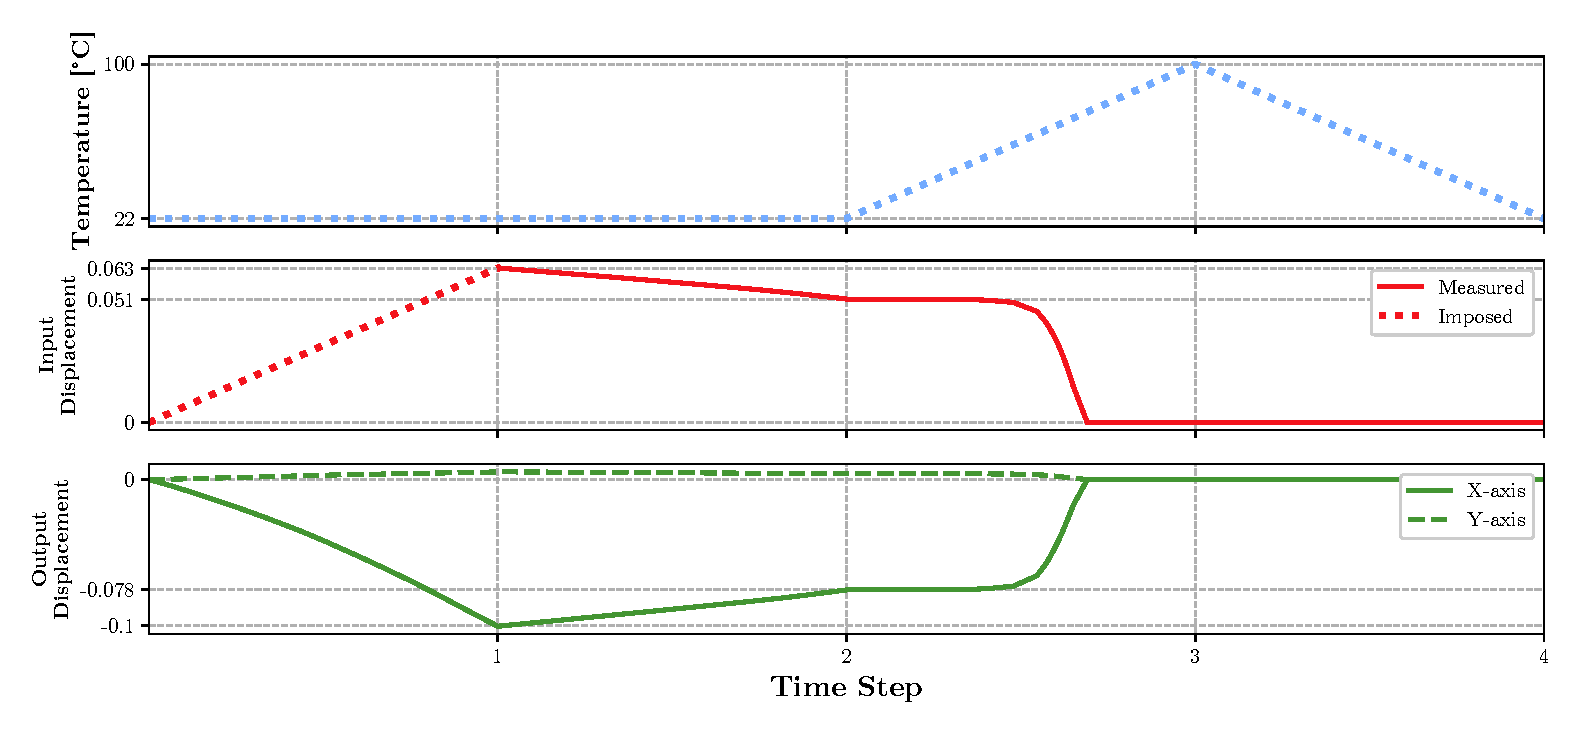
\includegraphics[width=\textwidth]{images/chap5/BM_Inverter30.eps}};
    \begin{scope}[x={(graph.south east)},y={(graph.north west)}]
    % \coordinate (ts0) at (1.54,7.6);
    % \coordinate (ts4) at (17.55,7.6);
    \coordinate (ts0) at (0.085,0.945);
    \coordinate (ts4) at (0.985,0.945);
    \coordinate (ts1) at ($ (ts0)!0.25!(ts4) $);
    \coordinate (ts2) at ($ (ts0)!0.5!(ts4) $);
    \coordinate (ts3) at ($ (ts0)!0.75!(ts4) $);
    \node[anchor=mid,inner sep=0] (ls0) at ($(ts0)!0.5!(ts1) + (0,0.05) $) {\fbox{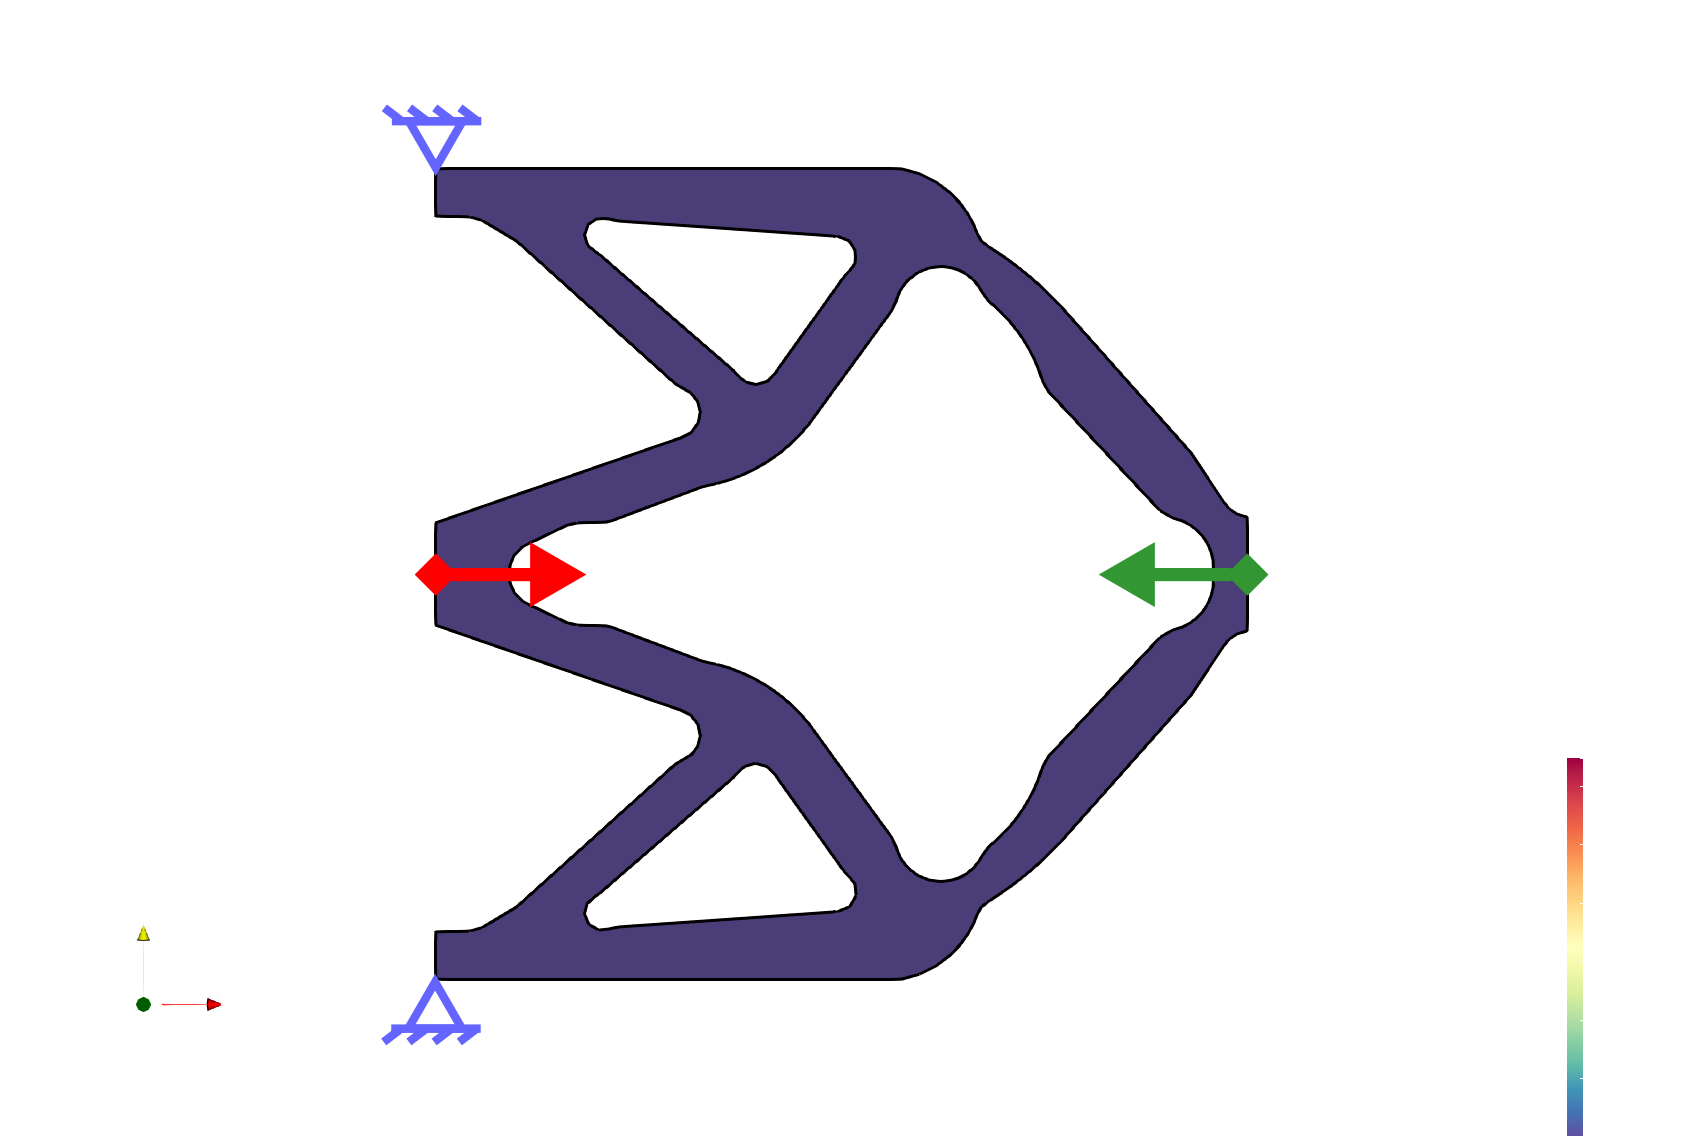
\includegraphics[height = 2cm,trim={11cm 3cm 13cm 3cm},clip]{images/chap5/Inverter_step0_v3.png}}};
    \draw[black, thick, -latex](ls0.west) to [bend right] (ts0);
    \node[anchor=mid,inner sep=0] (ls1) at ($(ts1)!0.5!(ts2) + (0,0.05) $) {\fbox{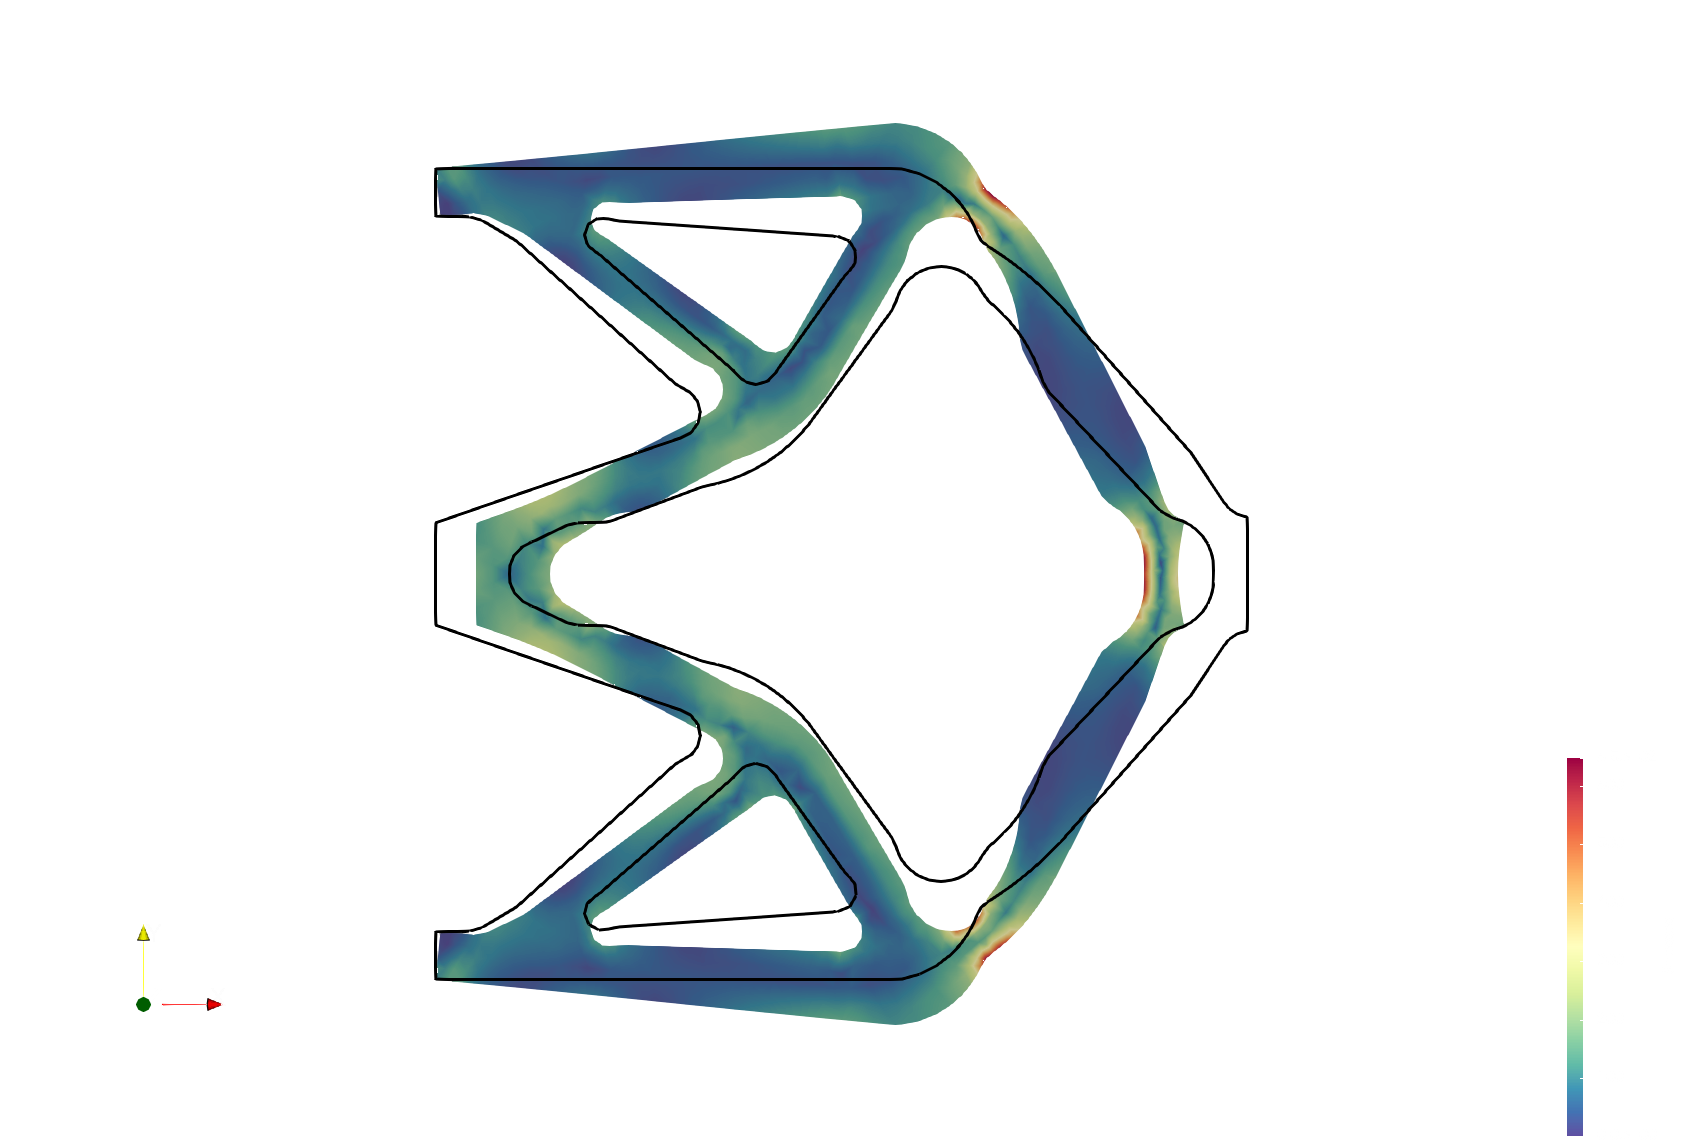
\includegraphics[height = 2cm,trim={11cm 3cm 13cm 3cm},clip]{images/chap5/Inverter_step1.png}}};
    \draw[black, thick, -latex](ls1.west) to [bend right] (ts1);
    \node[anchor=mid,inner sep=0] (ls2) at ($(ts2)!0.5!(ts3) + (0,0.05) $) {\fbox{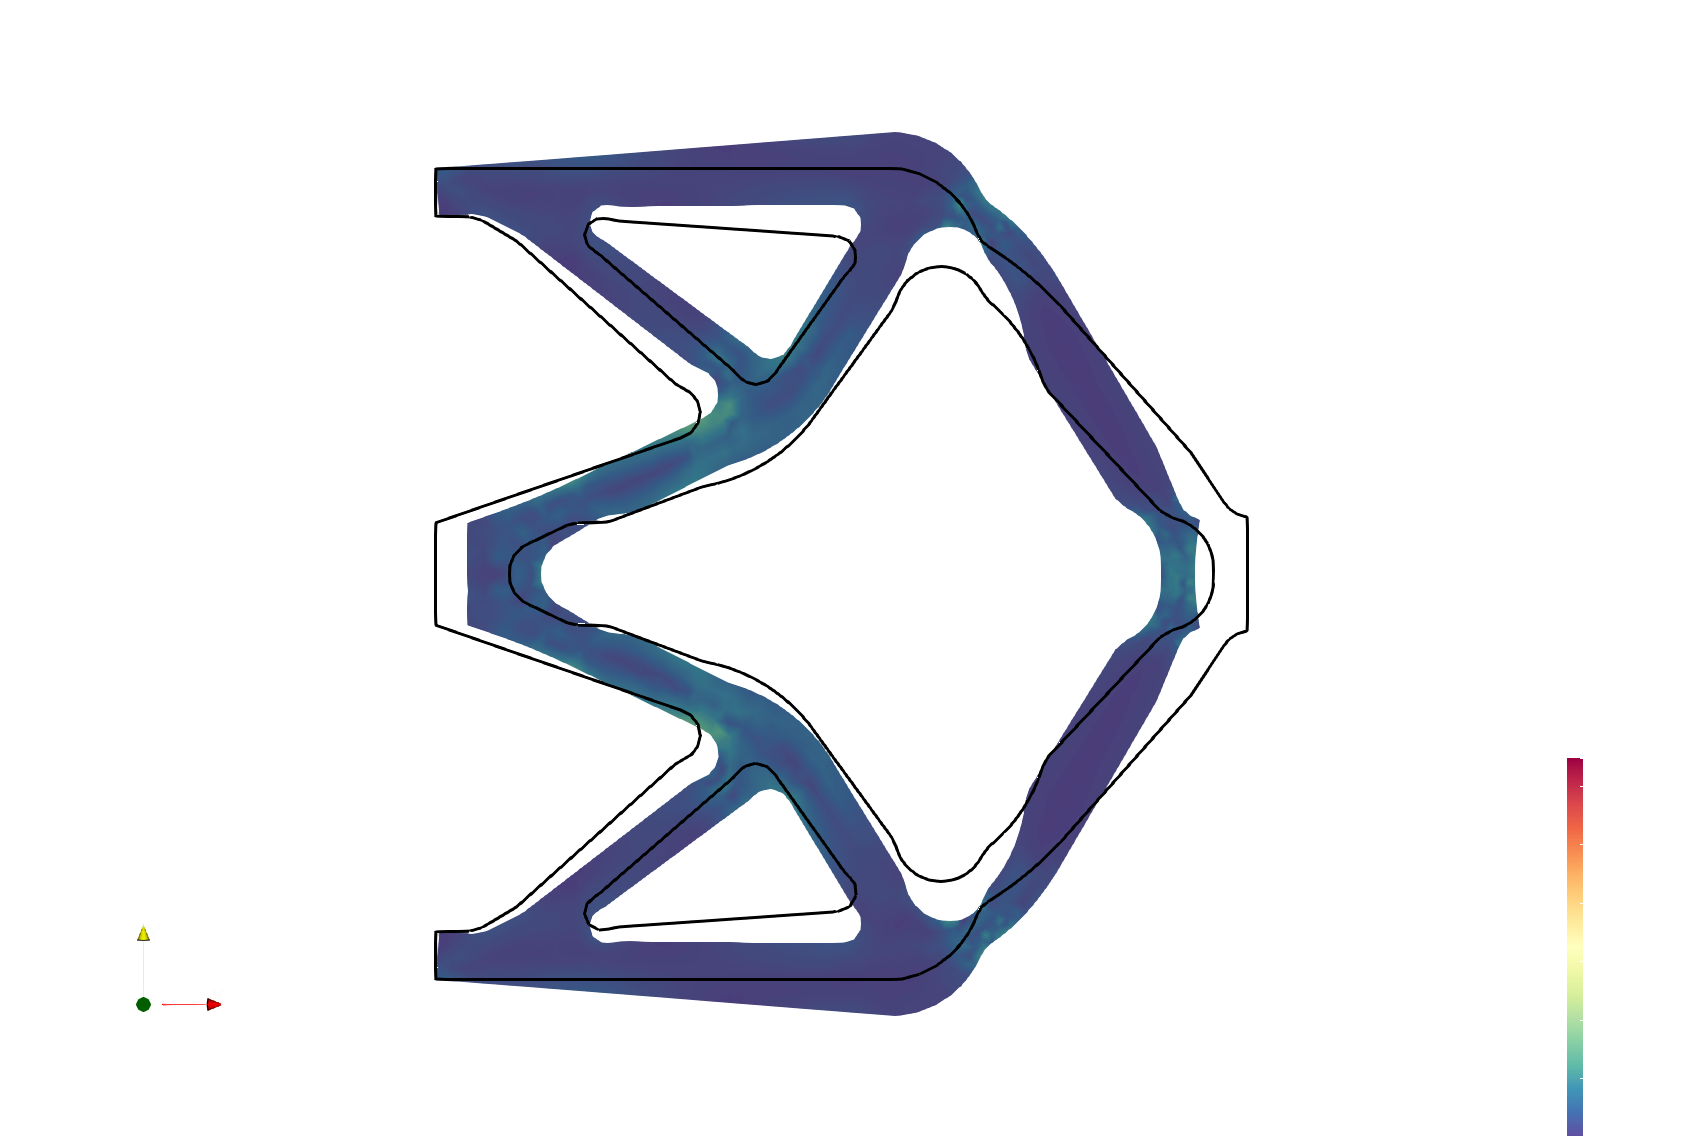
\includegraphics[height = 2cm,trim={11cm 3cm 13cm 3cm},clip]{images/chap5/Inverter_step2.png}}};
    \draw[black, thick, -latex](ls2.west) to [bend right] (ts2);
    \node[anchor=mid,inner sep=0] (ls3) at ($(ts3)!0.5!(ts4) + (0,0.05) $) {\fbox{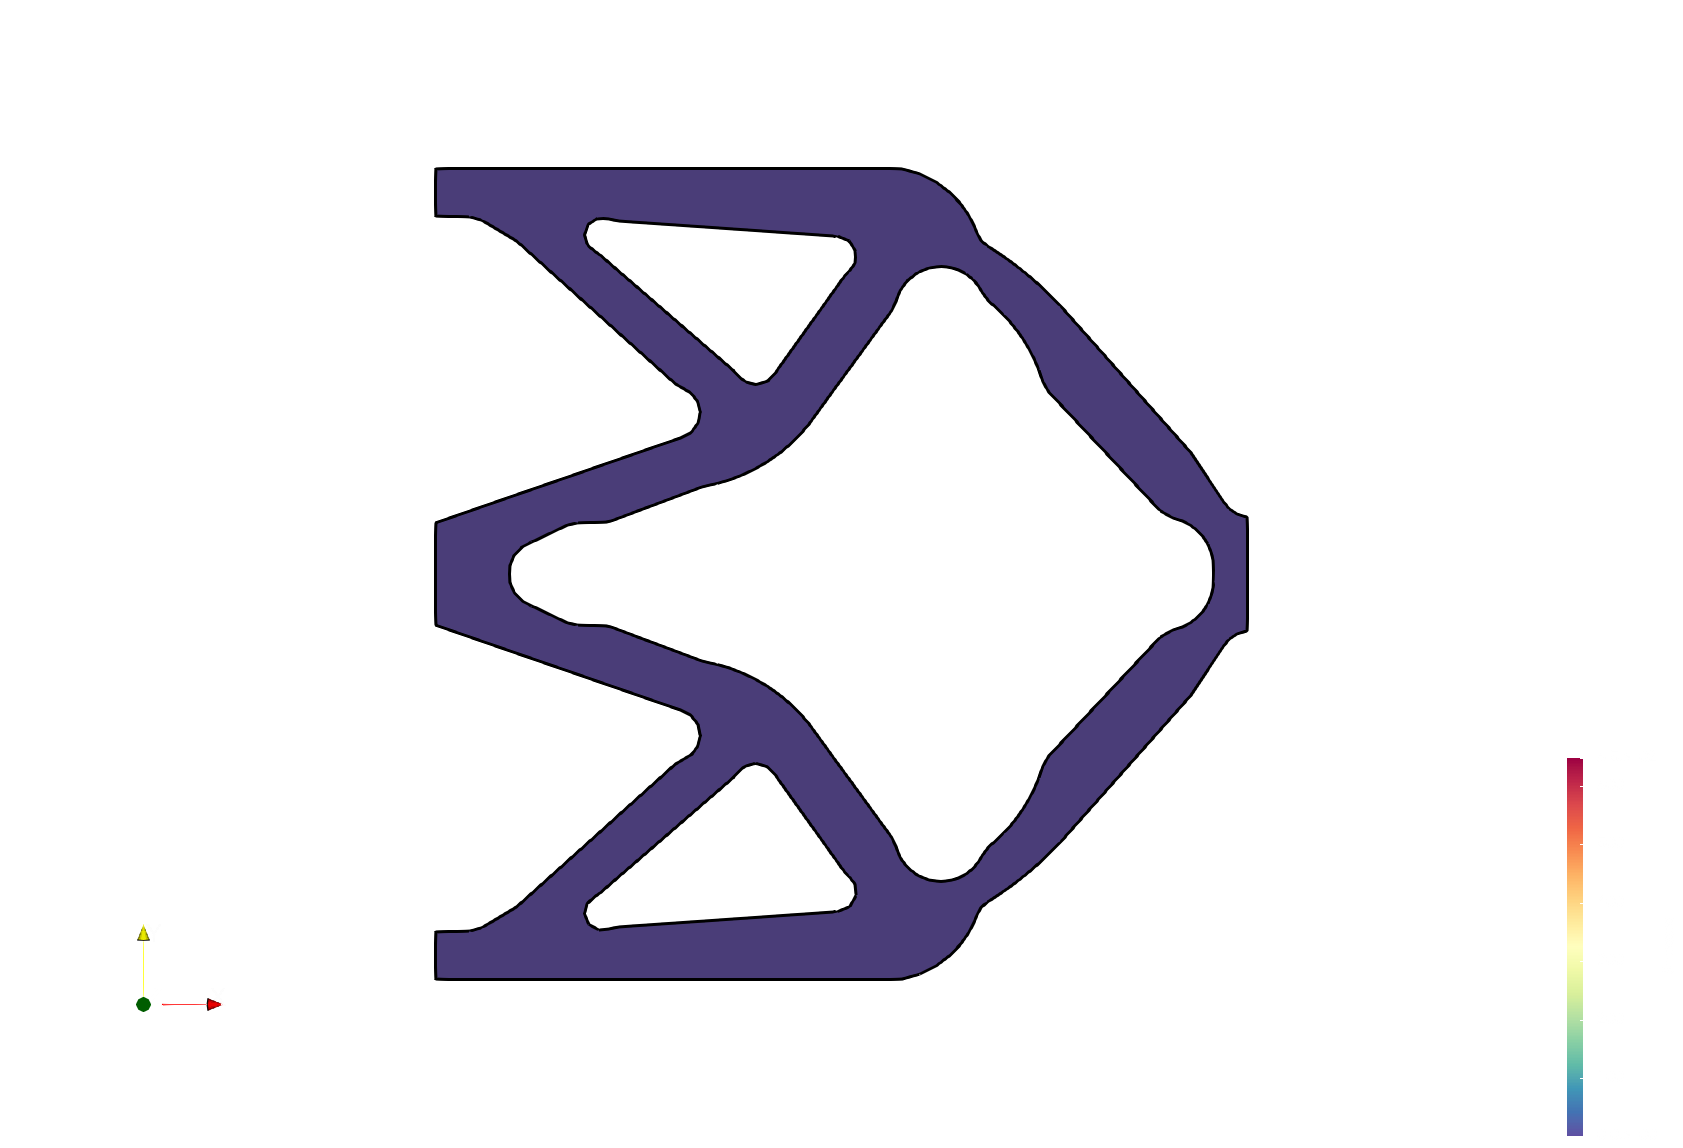
\includegraphics[height = 2cm,trim={11cm 3cm 13cm 3cm},clip]{images/chap5/Inverter_step0.png}}};
    \draw[black, thick, -latex](ls3.west) to [bend right] (ts3);
    \node[anchor=south east,inner sep=0] (ls0) at ($(ts4) + (0,0.015) $) {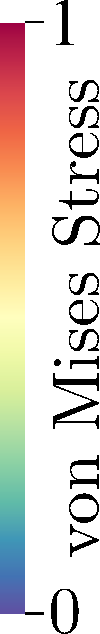
\includegraphics[height = 2.3cm]{images/chap5/Colorbar.pdf}};
    % \draw (0,0) node[circle, fill]{test};
    \filldraw ($ (ts0)!0.25!(ts4) + (0,-0.3)$) circle (1.5pt) node[anchor=north west] {$\epsilon_\text{loaded}$};
    \filldraw ($ (ts0)!0.5!(ts4) + (0,-0.35)$) circle (1.5pt) node[anchor=south west] {$\epsilon_\text{free}$};
    \filldraw ($ (ts0)!0.25!(ts4) + (0,-0.815)$) circle (1.5pt) node[anchor=south west] {$\varepsilon_\text{loaded}$};
    \filldraw ($ (ts0)!0.5!(ts4) + (0,-0.745)$) circle (1.5pt) node[anchor=south west] {$\varepsilon_\text{free}$};
    \end{scope}
    \end{tikzpicture}%
\end{document}

    \caption{Results of the shape memory effect simulation of the Inverter design. Here, the displacements are calculated relatively to the design domain size $L$. The displacements observed between time steps 1 and 2 show a strain retention of $\alpha_\varepsilon$ = 79.9\% confirming the presence of the shape memory effect.}
    \label{fig:InverterAnsysSimu}
\end{figure}

\subsection{A Qualitative Measure of the SME}
\subsection{Validation of the methodology}
\section{Heating Strategies}
\subsection{Induction Heating}
\section{Examples of Multi-Output Compliant SMA Actuators}
\section{Kirigami inspired SMA Actuators}
\section{Summary and Conclusion}
